%%=============================================================================
%% Methodologie
%%=============================================================================

\chapter{\IfLanguageName{dutch}{Methodologie}{Methodology}}
\label{ch:methodologie}

%% TODO: Hoe ben je te werk gegaan? Verdeel je onderzoek in grote fasen, en
%% licht in elke fase toe welke stappen je gevolgd hebt. Verantwoord waarom je
%% op deze manier te werk gegaan bent. Je moet kunnen aantonen dat je de best
%% mogelijke manier toegepast hebt om een antwoord te vinden op de
%% onderzoeksvraag.

In dit stuk van de bachelorproef zal men uitleggen hoe het onderzoek tot stand heeft gebracht. Men kan hierin waarnemen hoe men beslissingen heeft genomen omtrent specifieke eigenschappen van de verschillende AI-frameworks. Dit hoofdstuk is verdeeld is vier subsecties, elk van hen verdiept zich meer in hoe elk bepaald stuk van het onderzoek werd gerealiseerd.

\section{Voorbereiding}
Deze subsectie verdiept zich in hoe het toekomstig onderzoek werd uitgestippeld. Men ging verschillende toenaderingen zoeken om een AI-framework op een zo goed mogelijke manier te kunnen evalueren, dit is vervolgens het raamwerk dat werd gebruikt als aanpak in de evaluatie. Er werd ook een extra exploratief onderzoek verwezenlijkt om reeds uitgewerkte voorbeelden te achterhalen die gebruikt maakten van de concrete AI-frameworks. Op deze manier kon men snel testen of de frameworks de moeite waard zijn om deze verder te gebruiken in de proof-of-concept.
\newpage

\subsection{ Onderzoek naar AI-frameworks}
Bij het zoeken van de verschillende frameworks heeft men rekening gehouden met bepaalde criteria die invloed zouden kunnen hebben op het onderzoek:
\begin{itemize}
	\item De kost van het framework (betalend of gratis)
	\item Een mogelijke limiet op het aantal 'calls'
	\item De compatibiliteit met ARKit
	\item Documentatie
	\item Reeds uitgewerkte voorbeelden
\end{itemize}

In dit onderzoek werden 2 AI-frameworks onder de loep genomen, deze voldeden reeds aan alle criteria die werden opgesteld:

\begin{itemize}
	\item TensorFlow Lite (TensorFlow)
	\item CoreML (Apple)
\end{itemize}

De twee andere frameworks die ook werden besproken in de stand van zaken werden niet onderzocht, deze frameworks zijn immers betalend (Vuforia en Vision API). 

\subsection{Beoordelingstechnieken}
Om het juiste AI-framework te kiezen heeft men elk van hen op een grondige manier geëvalueerd. Om dit op een optimale manier te doen heeft men rekening gehouden met verschillende beoordelingstechnieken.

\subsubsection{Functionaliteit}
De eerste factor waar men rekening mee heeft gehouden is het feit of het AI-framework wel degenlijk deed wat er gevraagd werd. Om de frameworks op een zo divers mogelijk manier te kunnen testen heeft men verschillende soorten AI-eigenschappen getest:
\begin{itemize}
	\item Objectdetectie
	\item Menssegmentatie
	\item Luchtsegmentatie 
	\item Segmentatie binnen gebouwen
\end{itemize}
Segmentatie is het opsplitsen van een bepaald beeld in verschillende segmenten. Op deze manier zou het AI-framework bijvoorbeeld muren en grond van elkaar kunnen onderscheiden. De combinatie van objectdetectie en segmentatie is van zeer groot belang binnen deze bachelorproef, zo kan men vervolgens verschillende soorten objecten van elkaar onderscheiden en bepalen waar die zich juist bevinden. Deze uitvoering werd reeds uitgewerkt door 'Gestalt Robotics', een robot zal door deze implementatie op een correctie manier door het fabrieksgebouw bewegen.

\begin{figure}[H]
	\centering
	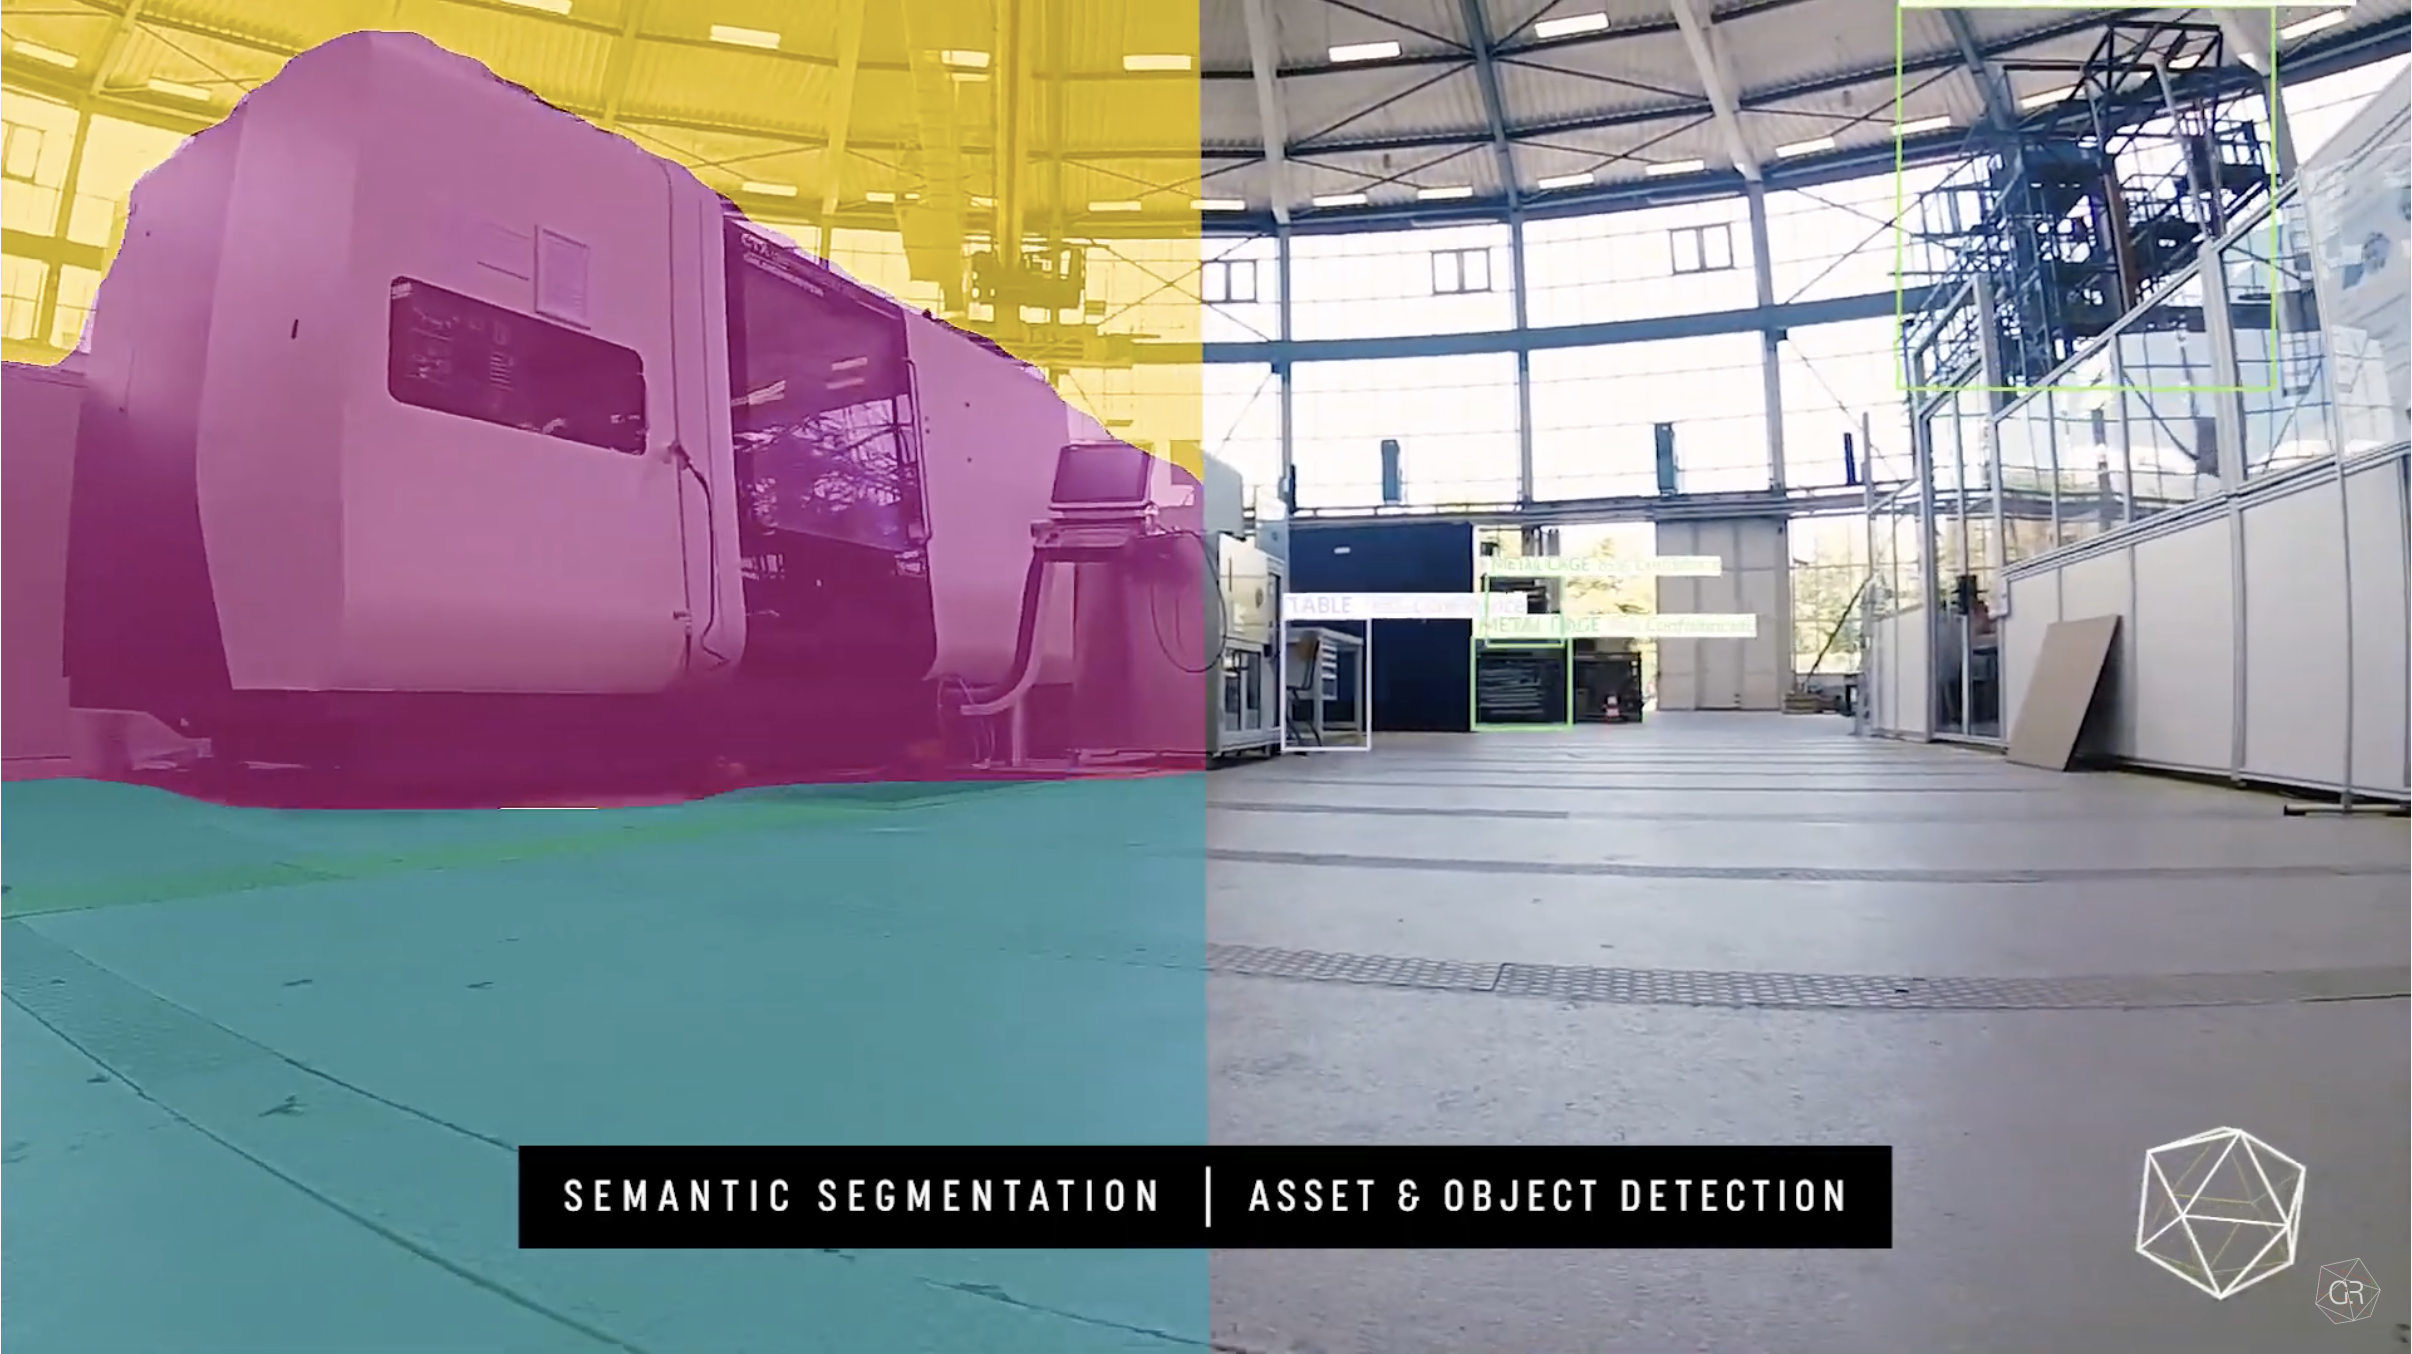
\includegraphics[scale=0.3]{SemanticSegmentation_ObjectDetection.png}
	\caption{Voorbeeld segmentatie + objectdetectie \autocite{Gestalt2019}}
\end{figure}

\subsubsection{Correctheid}
De 2de en meest cruciale factor is de correctheid van het AI-framework voor de verschillende soorten AI-eigenschappen. Het is belangrijk dat het framework betrouwbaar is en dus geen foute oplossing zal terug geven, anders zal dit verkeerd doorgegeven worden aan de visuele kant van de applicatie en zal de route verkeerd worden aangegeven. Om de correctheid van elk AI-framework te testen heeft men opnieuw de diverse AI-eigenschappen onder de loep genomen.

\subsubsection{Correctheid - 1.  Objectdetectie}
Om de objectdetectie te evalueren heeft men geobserveerd of het framework de juiste positie van het gerelateerde object aangeeft , alsook het percentage dat de correctie voorstelt werd in acht gehouden. Dit proces werd 29 keer herhaald, de resultaten werden gebundelend en geëvalueerd. 

\subsubsection{Correctheid - 2. Menssegmentatie}
Bij de evaluatie van de menssegmentatie werd er gekeken of het computer gegenereerde oppervlak overeen kwam met de vorm van de daadwerkelijke persoon. De foute zones werden aangeduid met markeringen om een duidelijk overzicht te krijgen. Deze test werd ook 29 maal herhaald voor elk framework, de resultaten werden telkens naast elkaar gelegd. Om deze eigenschap te evalueren werd een puntensysteem toegepast, elke keer werd een punt uitgedeeld aan het framework die de persoon het beste kon omkaderen. Het framework die na de 29ste test het meeste punten had, werd verkozen als 'winnaar'.

\subsubsection{Correctheid - 3. Luchtsegmentatie}
Luchtsegmentatie werd op dezelfde manier beoordeeld als menssegmentatie. Deze twee segmentaties hebben een zeer gelijkaardige input en output, maar toch is er een groot verschil binnenin het framework. Het algoritme wordt op een andere manier getraind en zo is er toch een mogelijkheid dat deze twee segmentaties voor verschillende resultaten zorgen. Alsook werd deze 29 keer getest, het evaluatieproces werd op dezelfde manier uitgeoefend als bij menssegmentatie.

\subsubsection{Correctheid - 4. Segmentatie binnen gebouwen}
Segmentatie binnen gebouwen is de uitwerking die het meest gerelateerd is met de AI-output die voor deze bachelorproef van belang is. Het biedt namelijk de mogelijkheid om muren van grond te onderscheiden, dit is de hoofdreden waarom men AI in deze wayfinding-uitwerking wilt betrekken. Het is dus belangrijk dat deze AI-uitwerking grondig wordt geëvalueerd.

De evaluatie verliep als volgt, voor beide AI-frameworks werd op identiek dezelfde plaats de test uitgevoerd. Door de relevantie van de technologie was het moeilijk om twee uitgewerkte voorbeelden (TensorFlow Lite en CoreML) te vinden die dezelfde dataset gebruikten. Men heeft deze vergeleken door te kijken hoe goed beide frameworks in hun opzet zijn geslaagd. Dit proces werd alsook 29 keer herhaald, ook deze eigenschap werd op dezelfde manier geëvalueerd zoals lucht en menssegmentatie.
\begin{figure}[H]
	\centering
	\includegraphics[scale=0.3]{BeoordelingsTechnieken.png}
	\caption{Voorbeeld evaluatietechniek segmentatie binnen gebouwen}
\end{figure}

\subsubsection{Toegankelijkheid}
Een tweede belangrijke factor is de toegelankelijkheid van de AI-frameworks voor verschillende platformen. Zo is het belangrijk voor het bedrijf 'In The Pocket' dat ze een oplossing vinden dat schaalbaar is.

\subsubsection{Consistentie}
De derde en laatste factor die men onder de loep zal nemen is consistentie. Dit is een zeer cruciale factor binnen de wayfinding-context, het is belangrijk dat de eindgebruiker zich telkens op een correcte manier naar eindbestemming kan begeven met behulp van de toekomstige app, en niet in bv. 70 \% van de gevallen.

\subsection{Bepalen van optimaal AI-framework}
Het bepalen van welk AI-framework de optimale oplossing biedt werd gemaakt op basis van een overzicht van alle testen. Dit overzicht bevat staafdiagrammen die de resultaten van alle testen in kaart brengt, zo kan men rekening houden met de verschillende eigenschappen die elk framework te bieden heeft.

\chapter{\IfLanguageName{dutch}{Onderzoek}{Research}}
\label{ch:onderzoek}
In dit hoofdstuk zal de effectieve uitwerking van het onderzoek toegelicht worden. In het vorige hoofdstuk werd reeds het 'raamwerk' geschetst, dit hoofdstuk zal hier dus op verder gaan.In dit hoofdstuk zullen volgende zaken toegelicht worden:

\begin{itemize}
	\item Het bestuderen van de verschillende frameworks
	\item De AI-eigenschappen van elk framework valideren naargelang een vooropgestelde trainingset
	\item De resultaten bespreken voor elke AI-eigenschap
\end{itemize}

\section{De beproeving van de frameworks}
In deze sectie zullen de effectieve tests worden uitgevoerd, men zal steeds de resultaten van elk algoritme bespreken.

\subsection{Objectdetectie}

Zoals men eerder al heeft vermeld is objectdetectie een belangrijke factor binnen de wayfinding-context, men zal namelijk moeten weten waar elk object binnen een bepaalde kamer zich bevindt. Om dit op een goede manier te kunnen testen heeft men vijf verschillende objecten genomen en getest of men verschillende waarnemingen kon constateren. Om de resultaten te kunnen meten heeft men gebruik gemaakt van twee verschillende applicaties, 'Fritz AI Studio' en 'TFL Detect', beide applicaties werden uitgevoerd op een iPhone 11 (camera: 12MP). Beide frameworks maakten immers gebruik van de COCO dataset.


\subsubsection{Tests}
	\begin{figure}[H]
		\centering
		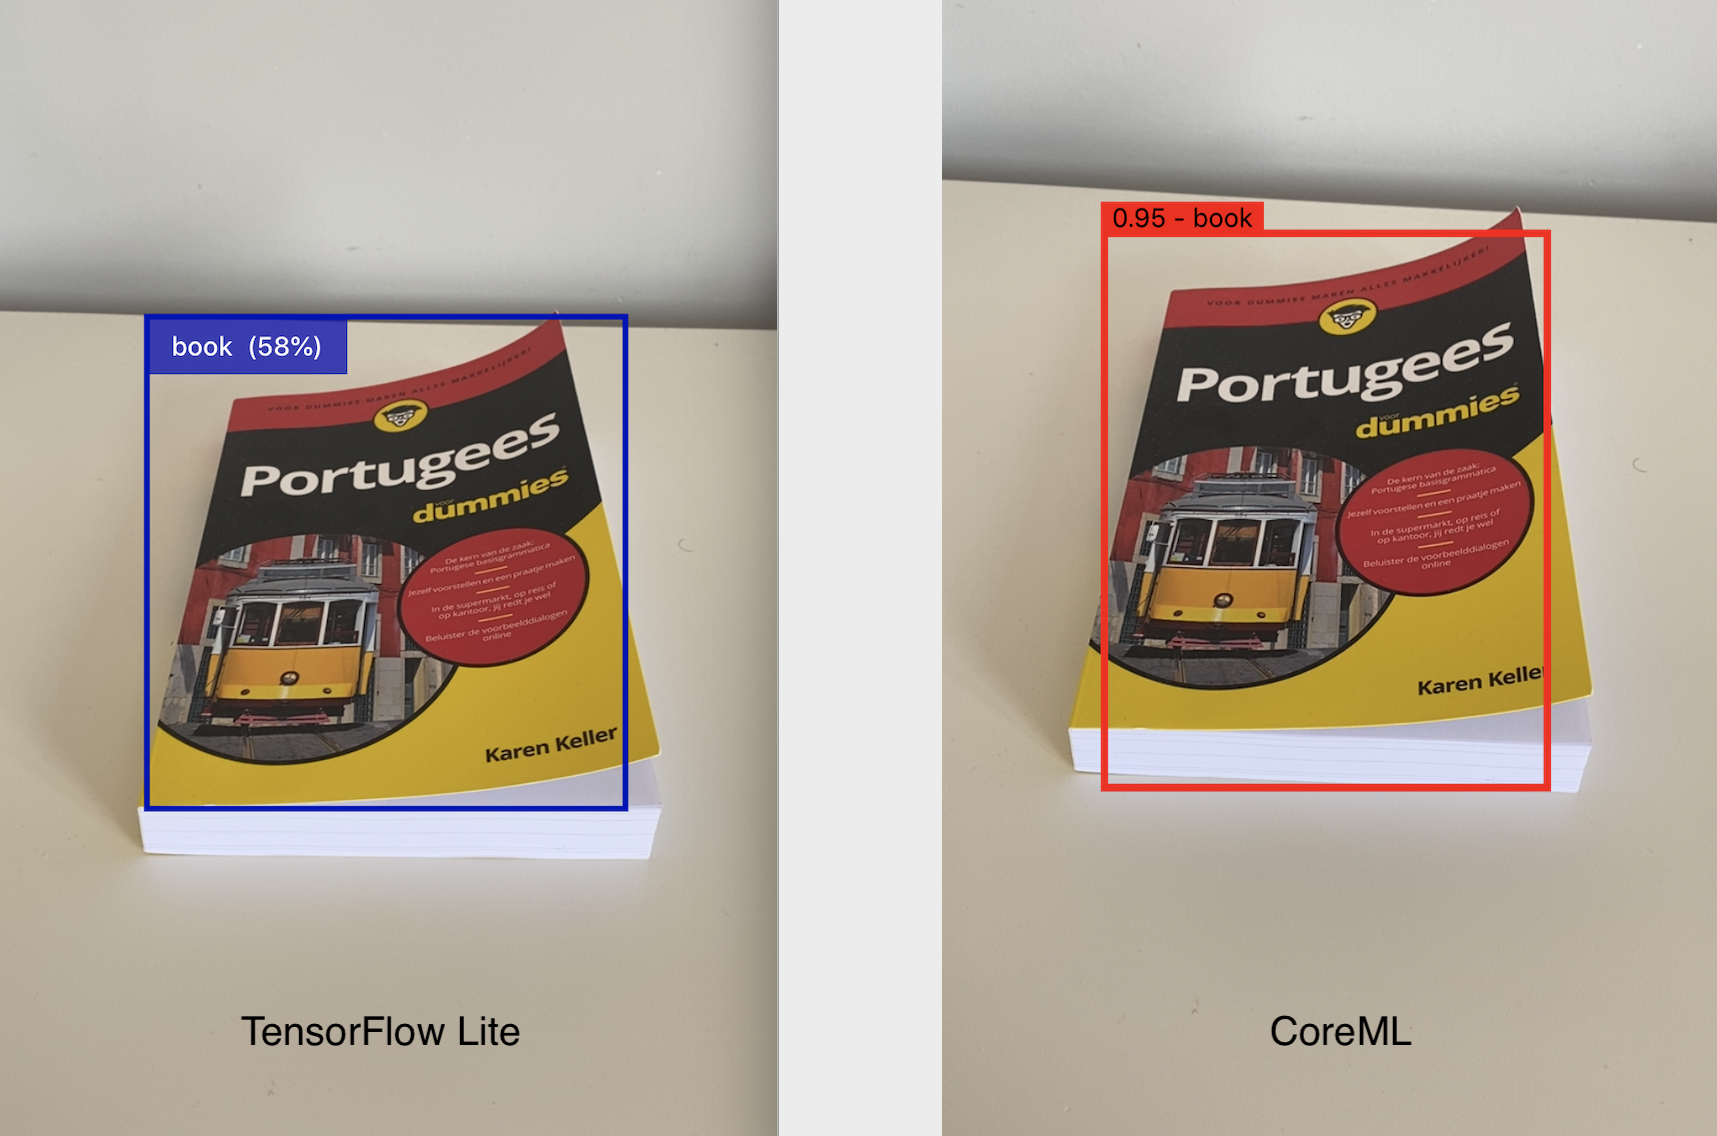
\includegraphics[scale=0.3]{ObjectDetection_Book.png}
		\caption{Test met boek, TensorFlow Lite (58\%) \& CoreML (95 \%)}
	\end{figure}
In de eerste objectdetectie-test kan men reeds waarnemen dat het boek beter wordt gedetecteerd door het CoreML-framework. Ten eerste wordt het boek nauwkeuriger aangeduid door de rechthoek, en ten tweede is het percentage veel beter. Het percentage dat de zekerheid aanduidt is namelijk 95 \% bij CoreML en 58 \% bij TensorFlow Lite. Dit redeneringsproces heeft men 29 keer herhaald.

\begin{figure}[H]
	\centering
	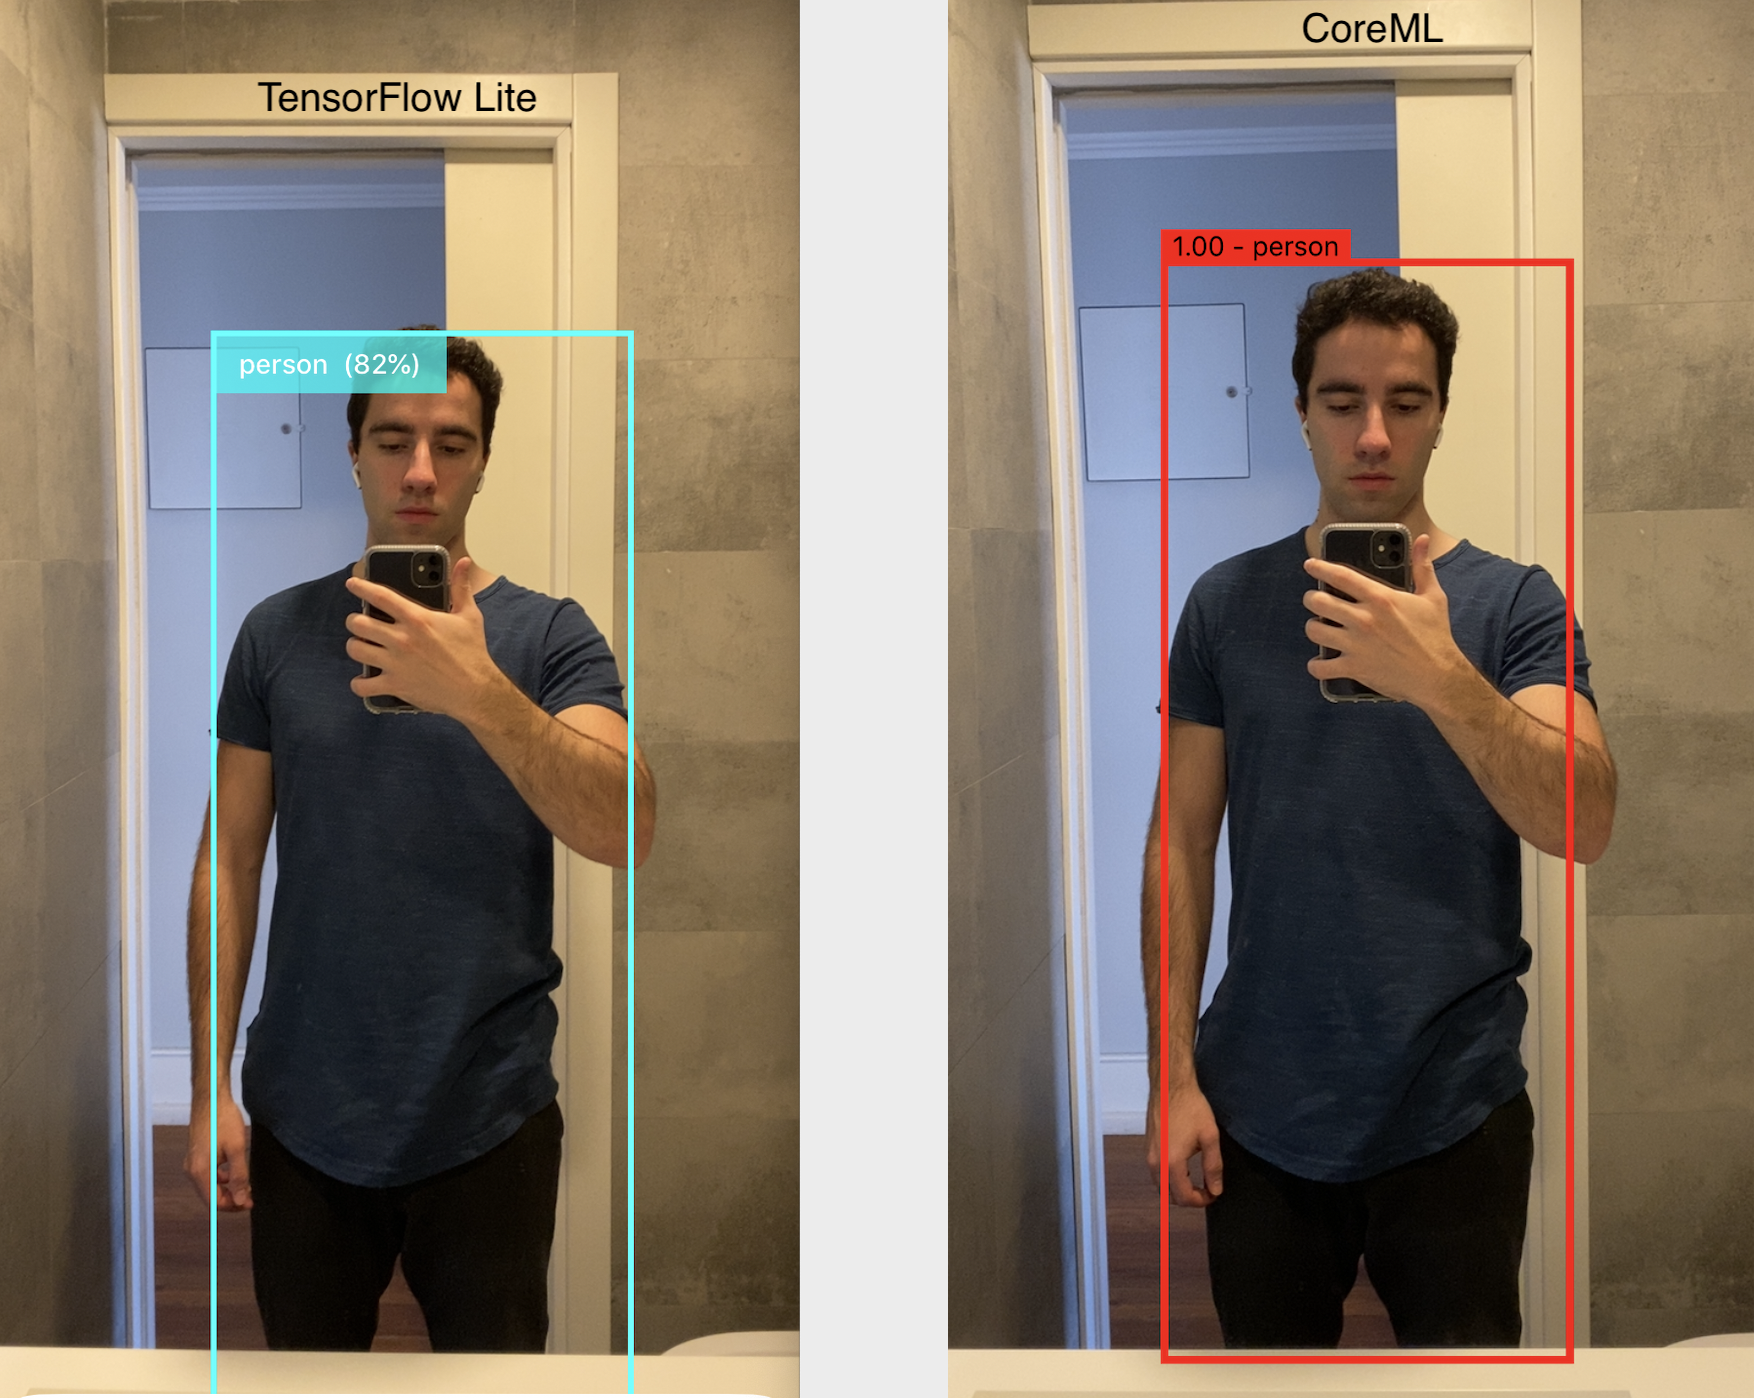
\includegraphics[scale=0.3]{ObjectDetection_Person.png}
	\caption{Test met persoon, TensorFlow Lite (82\%) \& CoreML (100 \%)}
\end{figure}
De tweede test toont nogmaals aan dat CoreML beter scoort. De persoon wordt veel exacter aangeduid met behulp van het vierkant. Het correctheidspercentage is nogmaals beter bij het CoreML-framework, men kan zelfs opmerken dat dit framework met 100\% kan zeggen dat het object een persoon is, dit resultaat is zeer opmerkelijk. Om te testen of de AI-frameworks consistent acteren heeft men dit redeneringsproces 29 maal herhaald.

\begin{figure}[H]
	\centering
	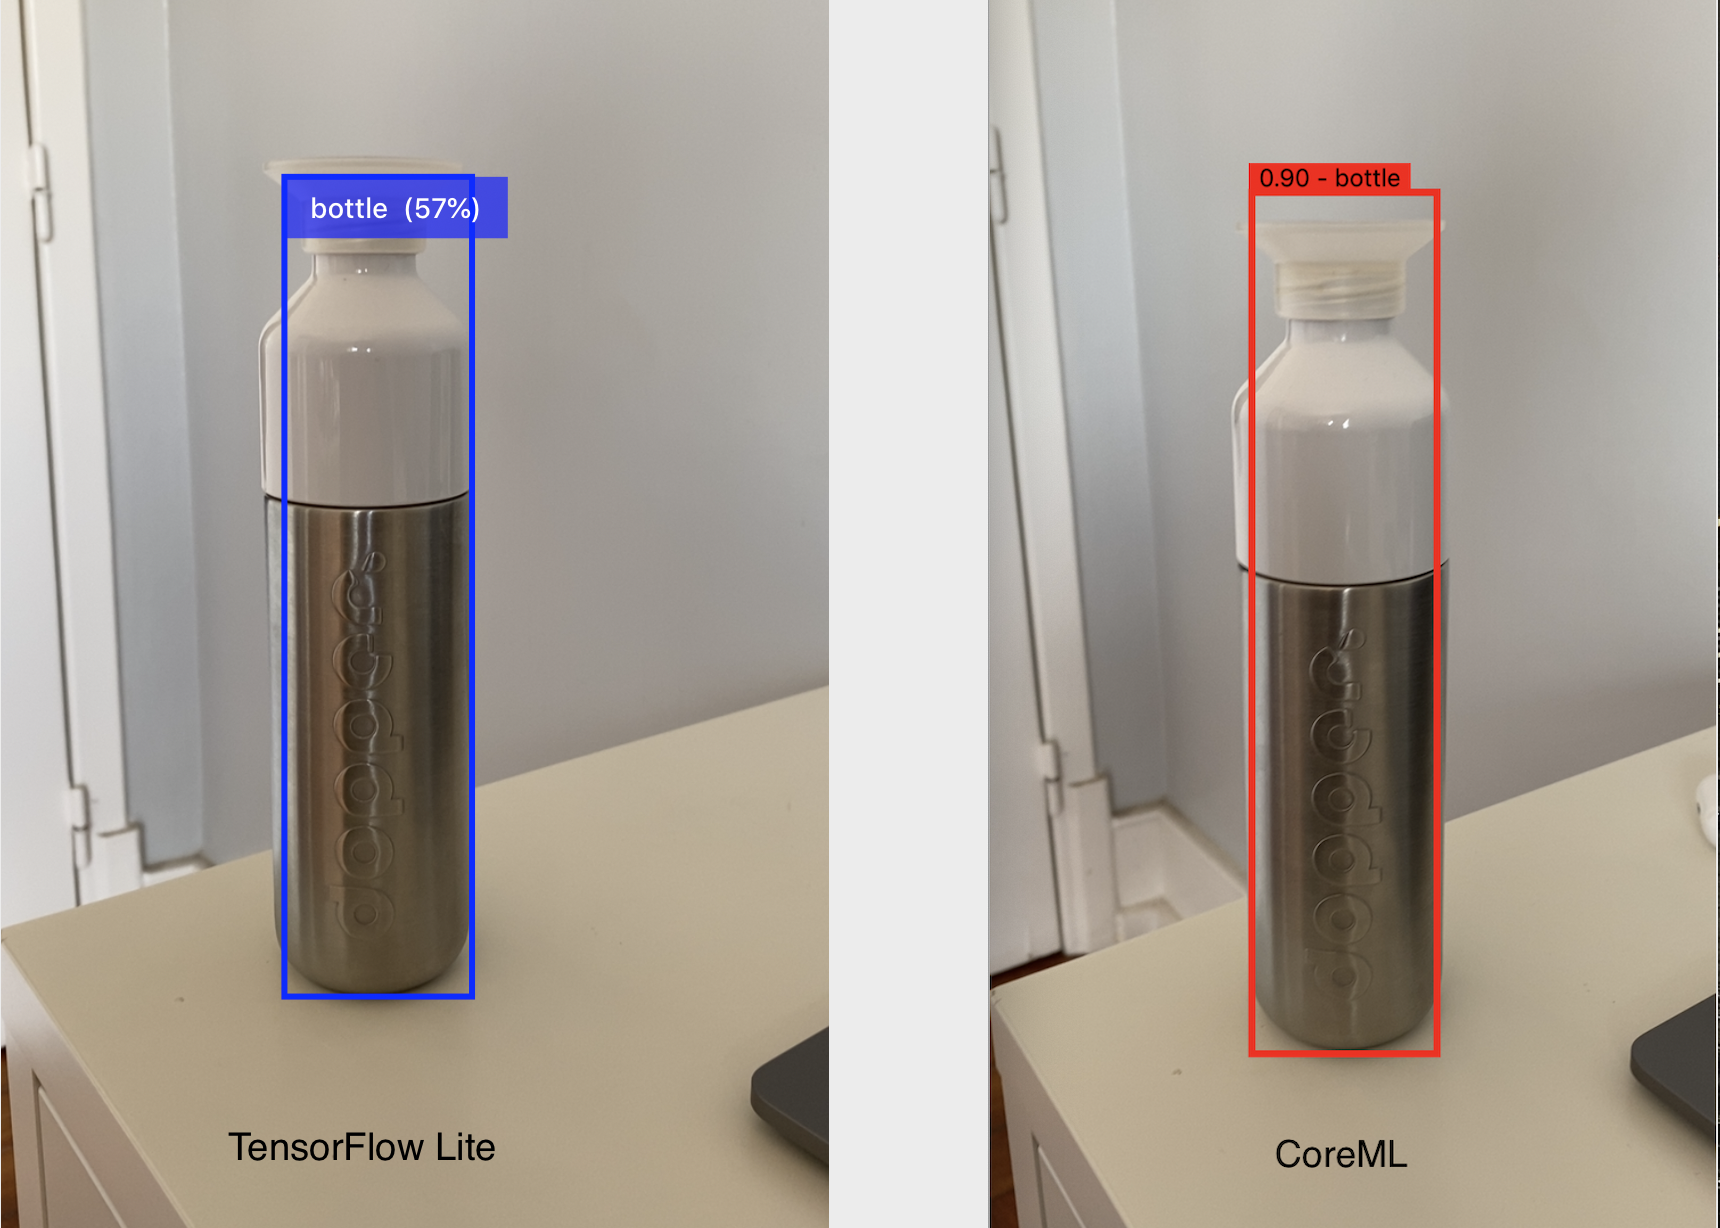
\includegraphics[scale=0.35]{ObjectDetection_Bottle.png}
	\caption{Test met waterfles, TensorFlow Lite (57\%) \& CoreML (90 \%)}
\end{figure}
Men kan opnieuw besluiten dat het framework van Apple een betere zaak doet om de waterfles te herkennen. Opnieuw kan men een significant correctheidsverschil opmerken tussen beide frameworks. CoreML kan in dit geval men bijna 30 \% meer zekerheid zeggen dat het vertoonde object een fles is. Ook voor dit object werd deze test 29 maal herhaald.
\begin{figure}[H]
	\centering
	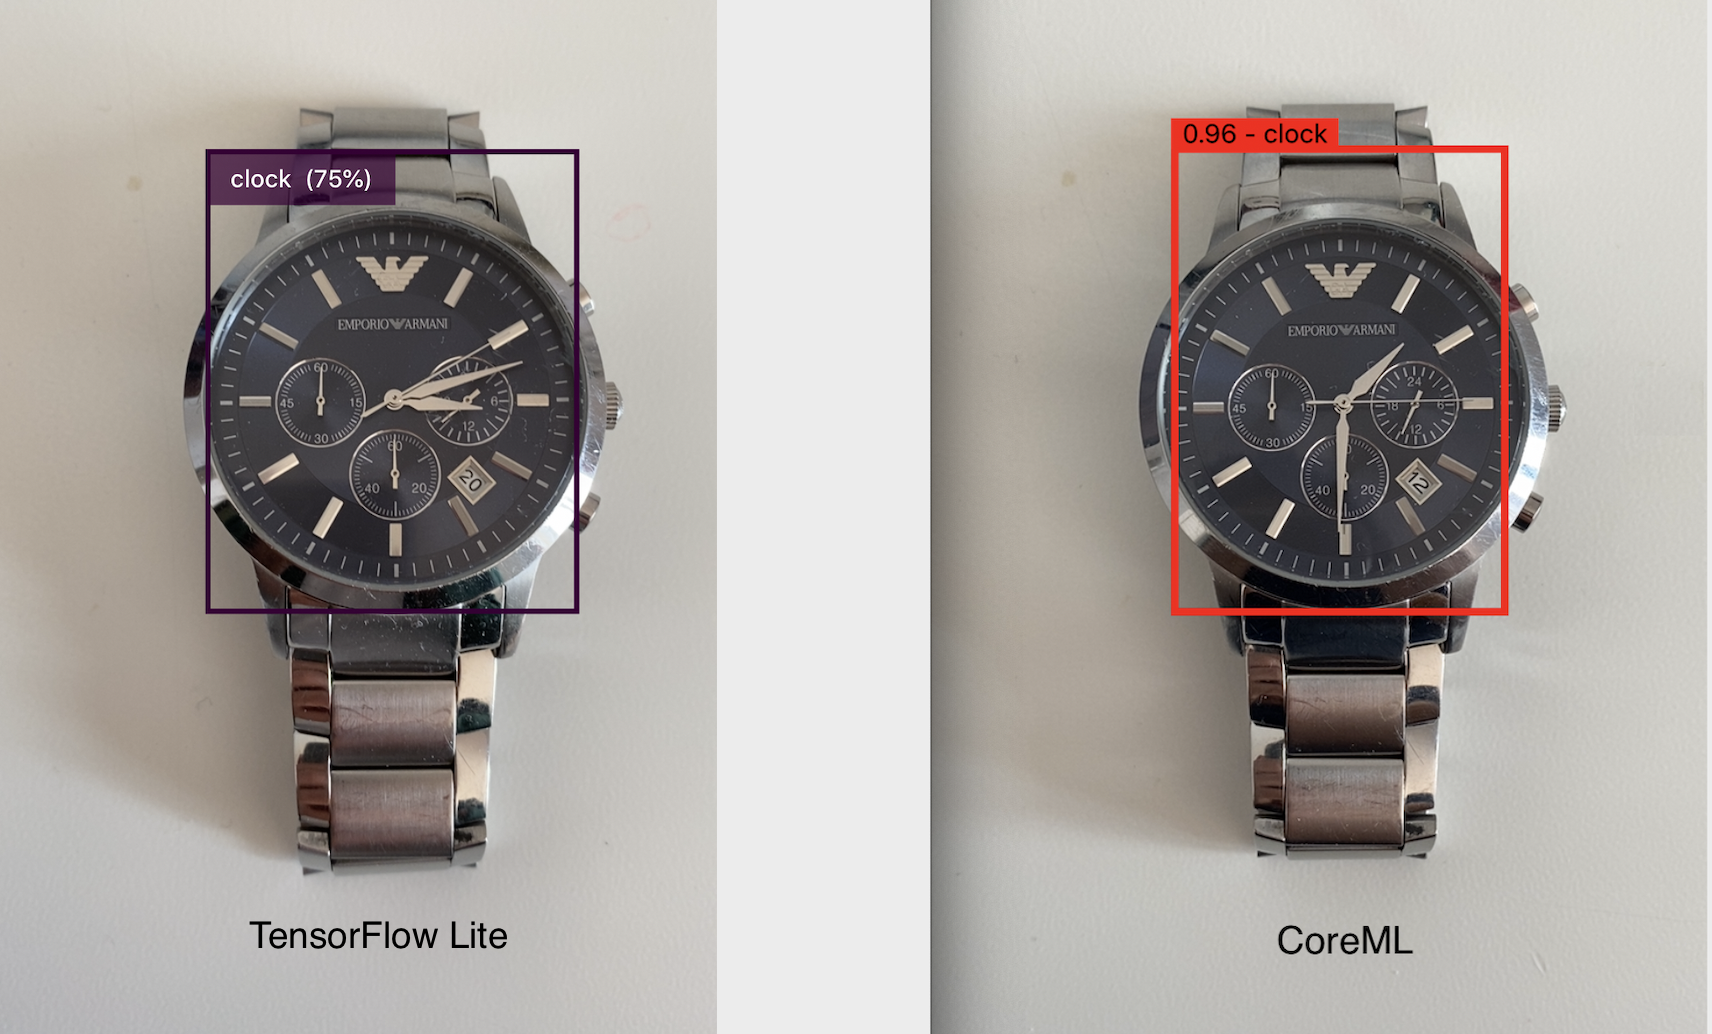
\includegraphics[scale=0.38]{ObjectDetection_Clock.png}
	\caption{Test met horloge, TensorFlow Lite (75 \%) \& CoreML (96 \%)}
\end{figure}
Andermaal kan men waarnemen dat het CoreML-framework betere resultaten levert als TensorFlow Lite, men kan in dit geval wel opmerken dat de detectie a.d.h.v het vierkant nauwkeuriger werd uitgevoerd door het TensorFlow Lite-framework. Opnieuw kan men een nauwkeurigheidsverschil opmerken van meer dan 20 \%. Dit redeneringsproces werd ook 29 maal herhaald om te achterhalen of de resultaten wel consistent zijn.

\begin{figure}[H]
	\centering
	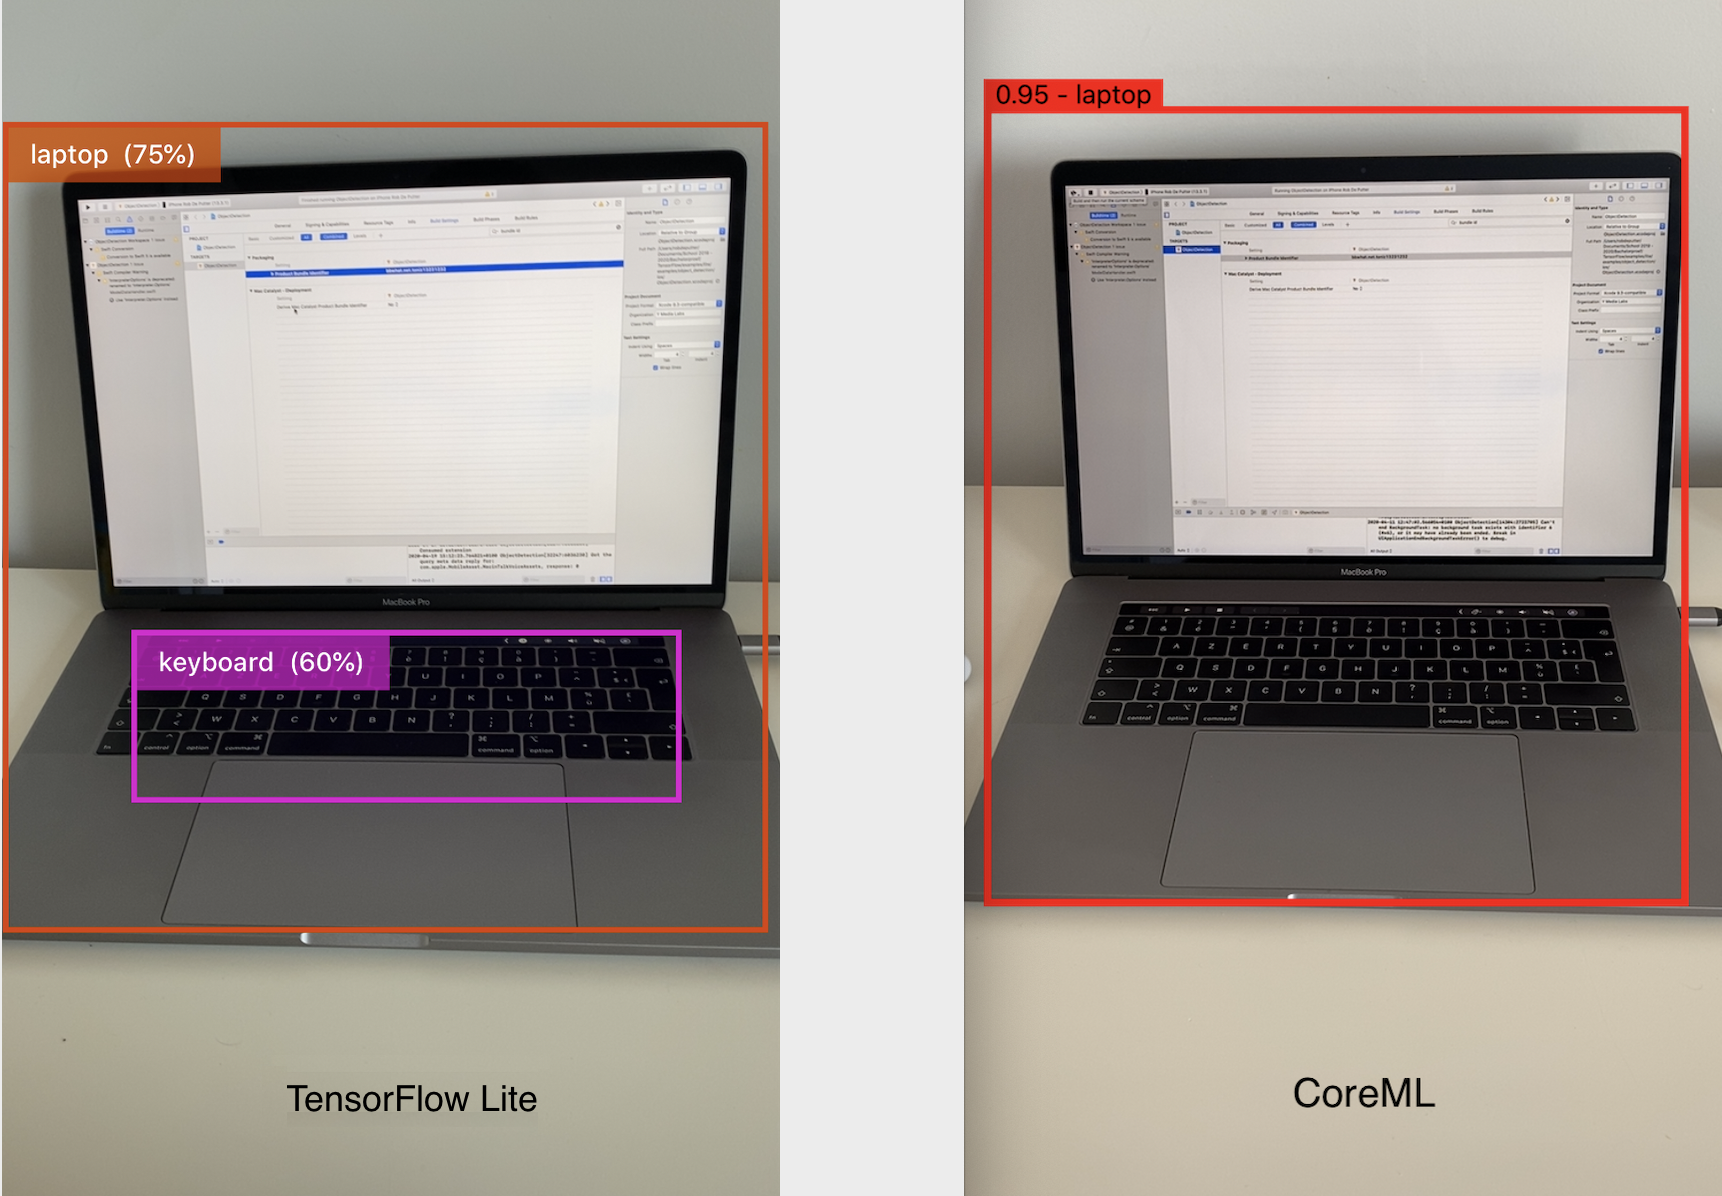
\includegraphics[scale=0.38]{ObjectDetection_Laptop.png}
	\caption{Test met laptop, TensorFlow Lite (75 \%) \& CoreML (95 \%)}
\end{figure}
De laatste test verschilt van de anderen, men kan namelijk bemerken dat TensorFlow Lite het toestenbord kan bespeuren, terwijl CoreML niet in staat is om dit te doen. De nauwkeurigheid kent wel lagere cijfers, opnieuw is er een verschil van 20 \% op vlak van accuraatheid. Alsook de laptoptest werd 29 maar herhaald. 
	

\subsection{Menssegmentatie}
De tweede AI-eigenschap die men getest heeft is menssegmentatie, in deze eigenschap zal men de volledige foto gaan onderzoeken of er zich mensen in begeven. Indien er zich mensen in het beeld bevinden zal het algoritme deze aanduiden door een bepaald kleuroppervlak over deze objecten te plaatsen. De resultaten werden bekomen door gebruik te maken van de 'Fritz AI Studio' applicatie op twee verschillende apparaten, namelijk een iPhone 11 (camera: 12MP) (iOS) en een Huawei P20 Lite (camera: 16MP) (Android). In de documentatie van de 'Fritz AI Studio' applicatie kan men opmerken dat de Android-variant gebruik maakt van TensorFlow Lite en de iOS-variant CoreML utiliseert. Deze beide frameworks gebruiken hetzelfde voorgetrainde model, dit werd samengesteld door Fritz AI.

\newpage
\subsubsection{Test}

\begin{figure}[H]
	\centering
	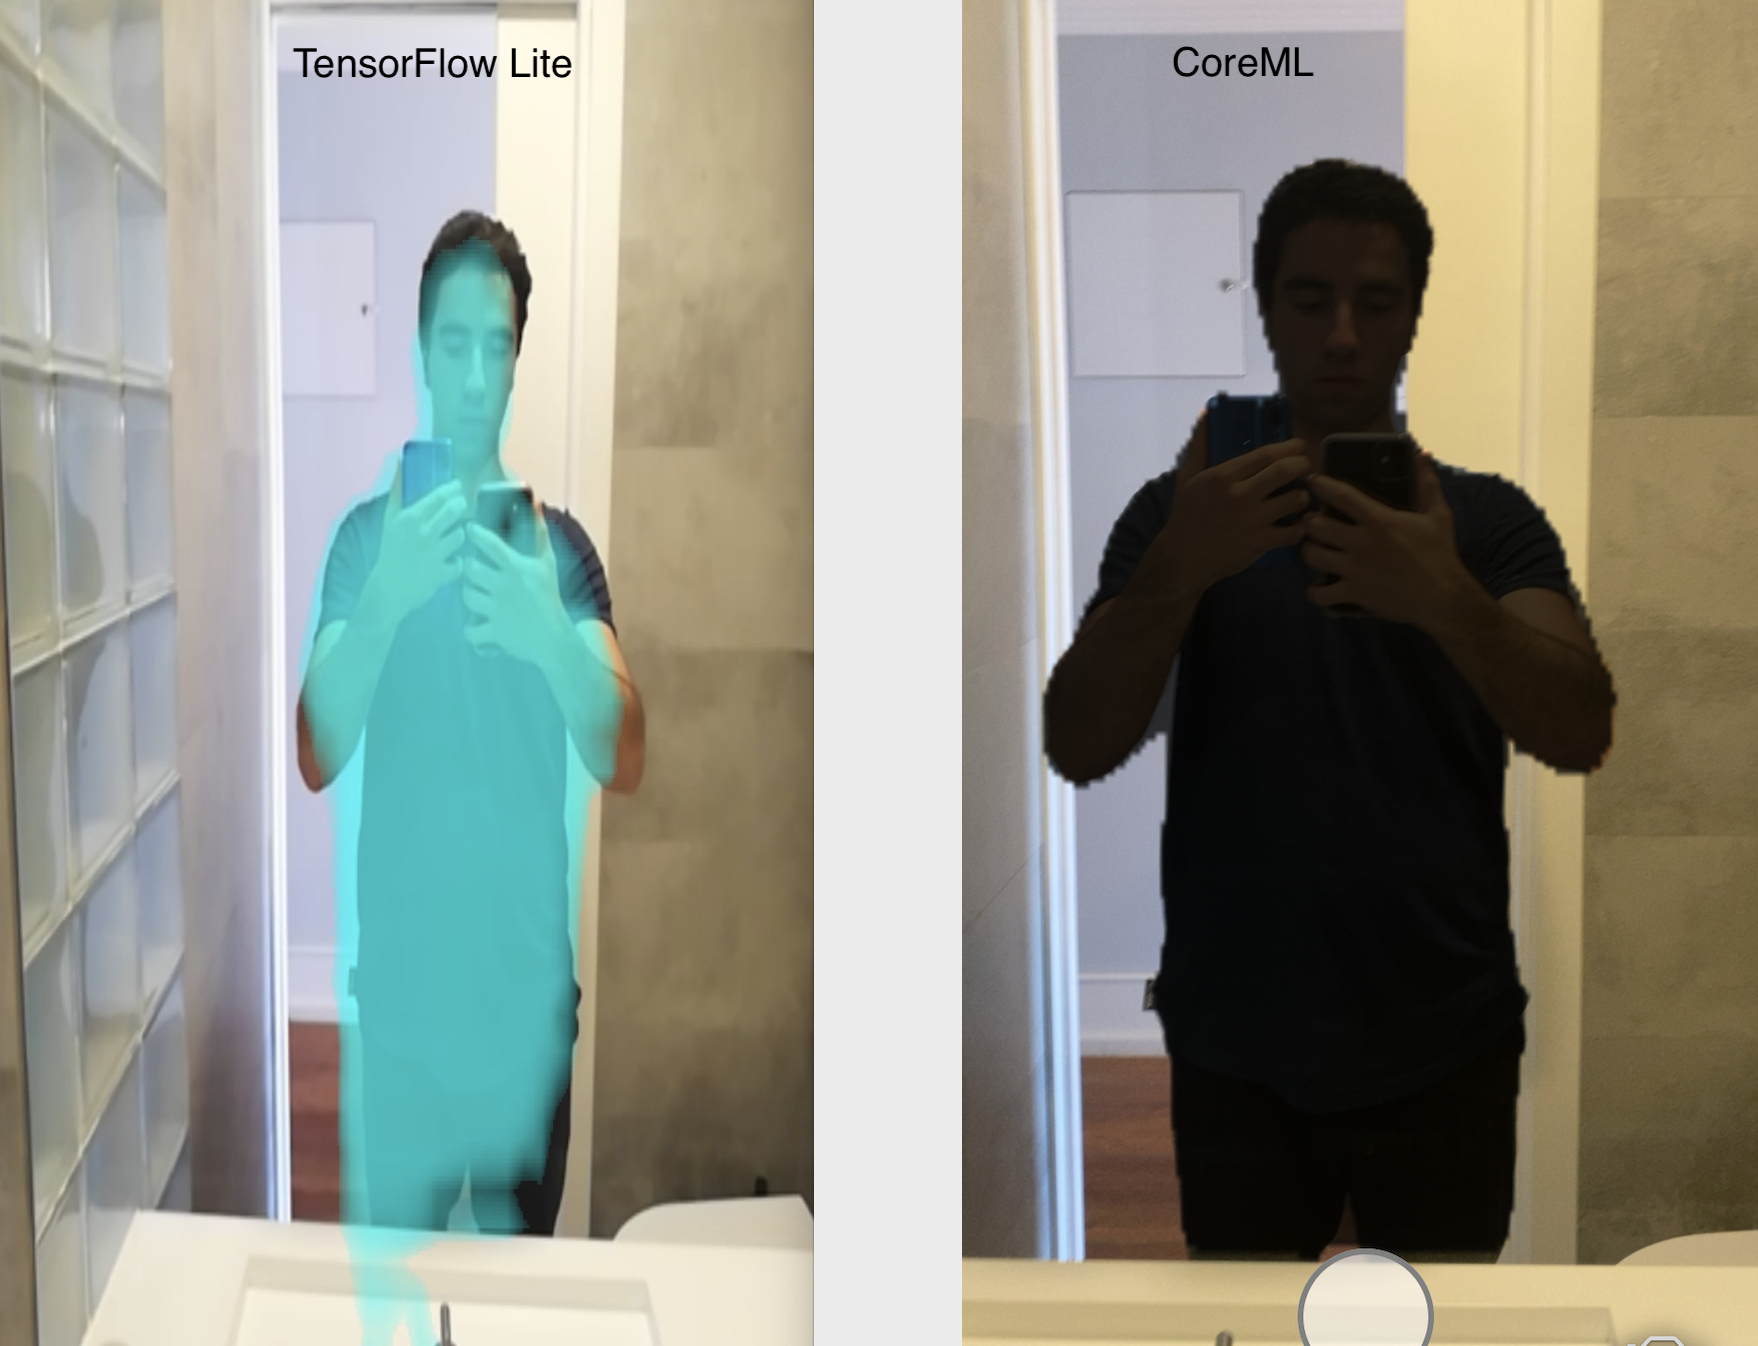
\includegraphics[scale=0.4]{PeopleSegmentation.png}
	\caption{Test menssegmentatie, zonder foutaanduiding}
\end{figure}
Uit de resultaten van deze test kan men opnieuw aanschouwen dat het CoreML-framework een veel betere uitslag levert dan TensorFlow Lite. Ondanks dezelfde dataset slaagt CoreML er in deze test toch in om de persoon in de afbeelding bijna 100 \% correct aan te duiden, de uitkomst van het andere framework is niet nauwkeurig en kent zelfs grove fouten. Men kan in deze test concluderen dat het CoreML-framework veel nauwkeuriger is. In de onderstaande afbeelding kan men de foute zones waarnemen, de rode vlaktes tonen aan waar de persoon niet werd gedetecteerd, maar wel was. Het gele gebied duidt de zones aan waar de persoon werd gedetecteerd, maar niet was. Dit visueel redeneringsproces werd 29 maal herhaald, telkens kreeg het framework met de minste foute zones een punt, het framework dat na de 29ste test het meeste punt haalde zou dit deelexperiment 'winnen'.

 De link tussen menssegmentatie en de wayfinding-context kan misschien ver te zoeken zijn, maar deze test zegt wel degelijk meer over de precisie van het AI-framework. Alsook is het mogelijk dat een groep mensen de weg kan versperren, in dit geval is het belangrijk dat deze groep wordt gedetecteerd door het algoritme, een zekere mensherkenning en detectie is dus zeker van belang.

\begin{figure}[H]
	\centering
	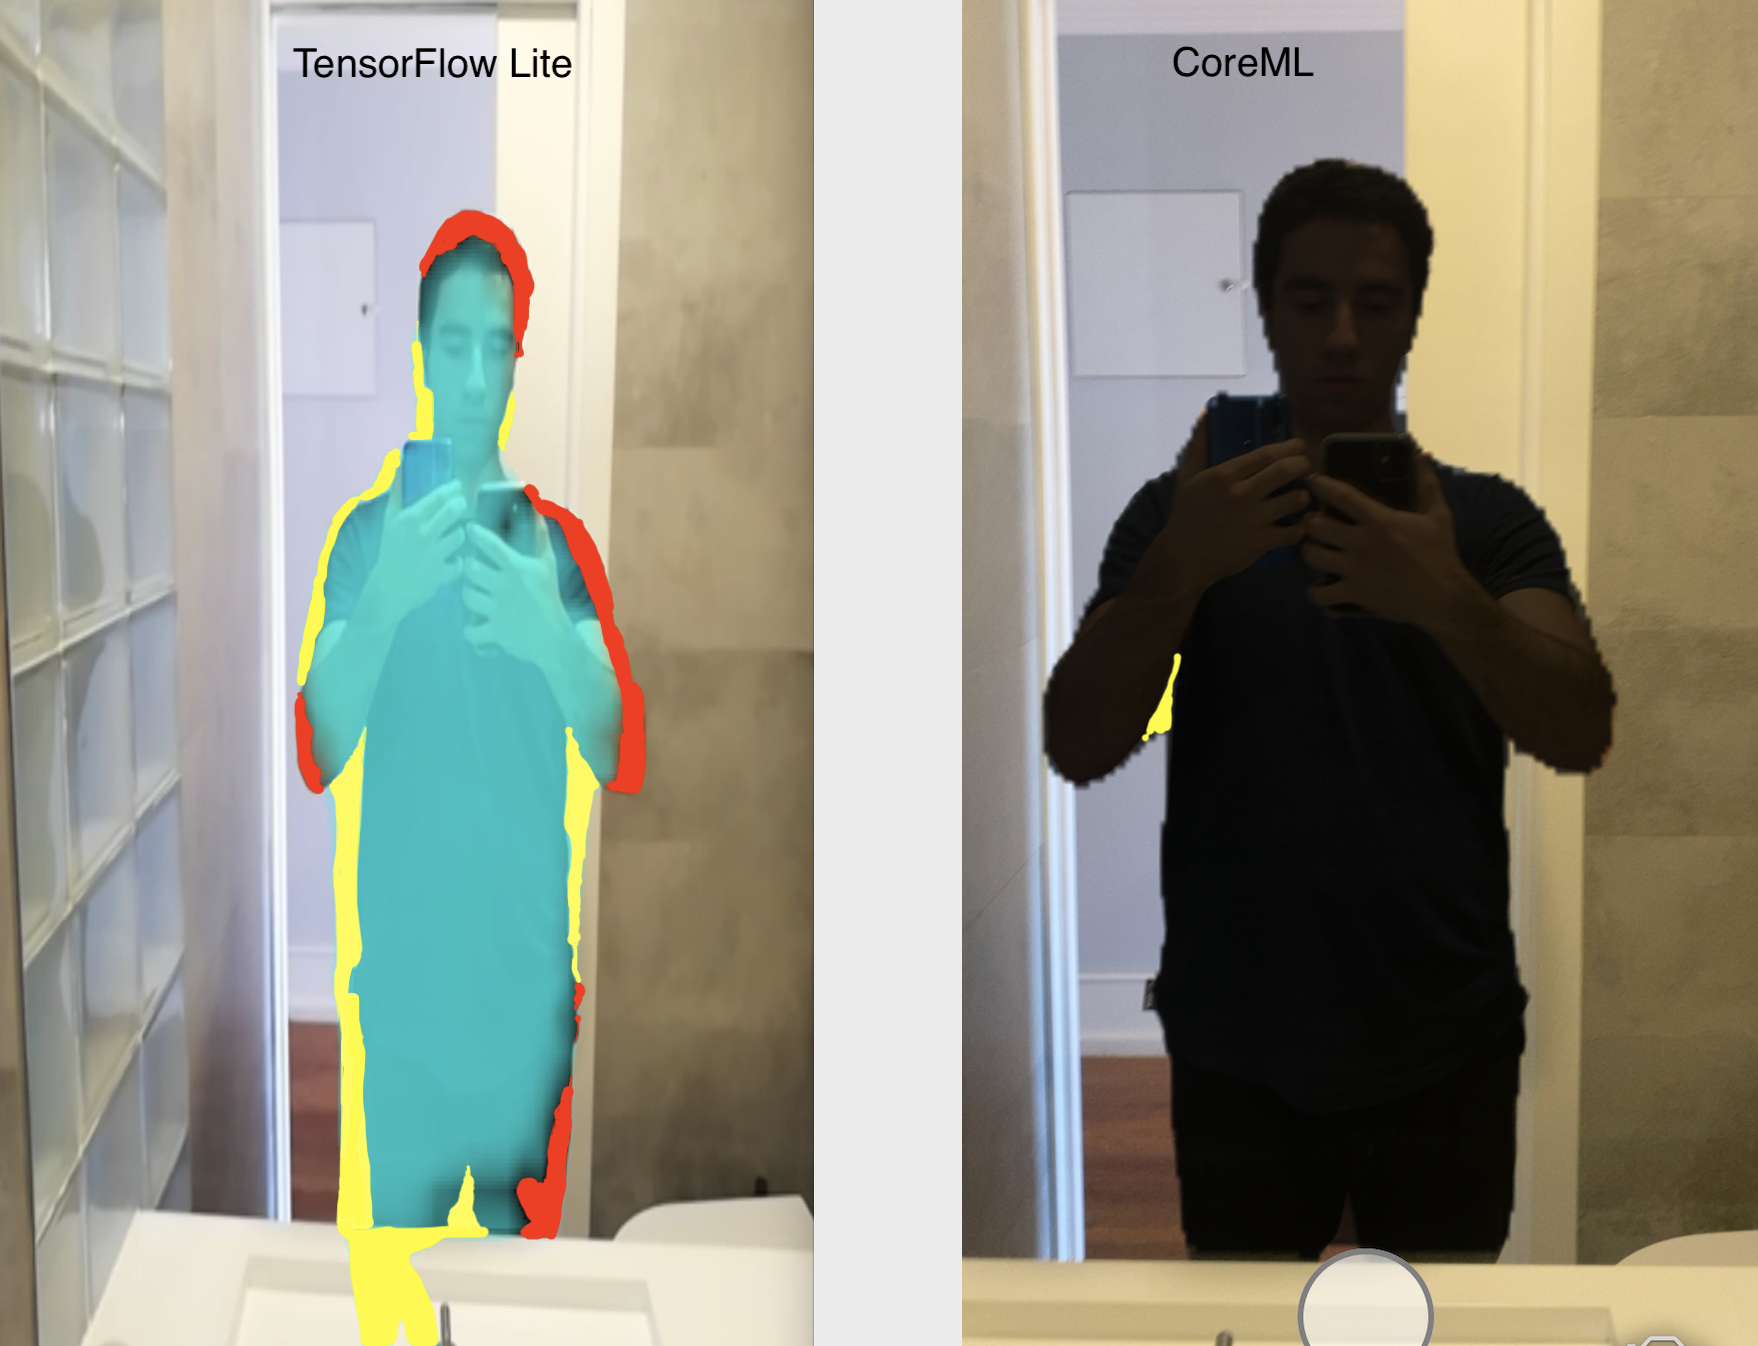
\includegraphics[scale=0.45]{PeopleSegmentation_MetFoutAanduiding.png}
	\caption{Test menssegmentatie, met foutaanduiding}
\end{figure}

\subsection{Luchtsegmentatie}
Om de AI-frameworks andermaal op nauwkeurig -en correctheid te testen, heeft men ervoor gekozen om ook luchtsegmentatie te observeren. Luchtsegmentatie zal net zoals menssegmentatie gekleurde vlekken plaatsen over de regio's waar men lucht detecteert. Alsook kan men bij deze AI-eigenschap denken dat dit geen direct verband heeft met de wayfinding context, maar toch geeft dit een extra beeld over hoe correct en nauwkeurig het AI-algoritme de verschillende vlakken kan onderscheiden. Zoals men eerder al aangaf in de methodologie zal men de foute zones aanduiden, het algoritme met het merendeel aan foute zones zal mogelijks niet worden geselecteerd als 'eindwinnaar'. Om deze test te kunnen uitvoeren werd de applicatie 'AI Fritz Studio' gebruikt, ook in dit onderzoek heeft men de applicatie beproeft op twee verschillende apparaten. Het CoreML-framework werd getest op een iPhone 11 (camera: 12MP), TensorFlow Lite werd uitgevoerd op een Huawei P20 Lite (camera: 16MP) (Android). Beide frameworks werden getrained met een dataset die werd opgesteld door Fritz AI.

\newpage
\subsubsection{Test}
\begin{figure}[H]
	\centering
	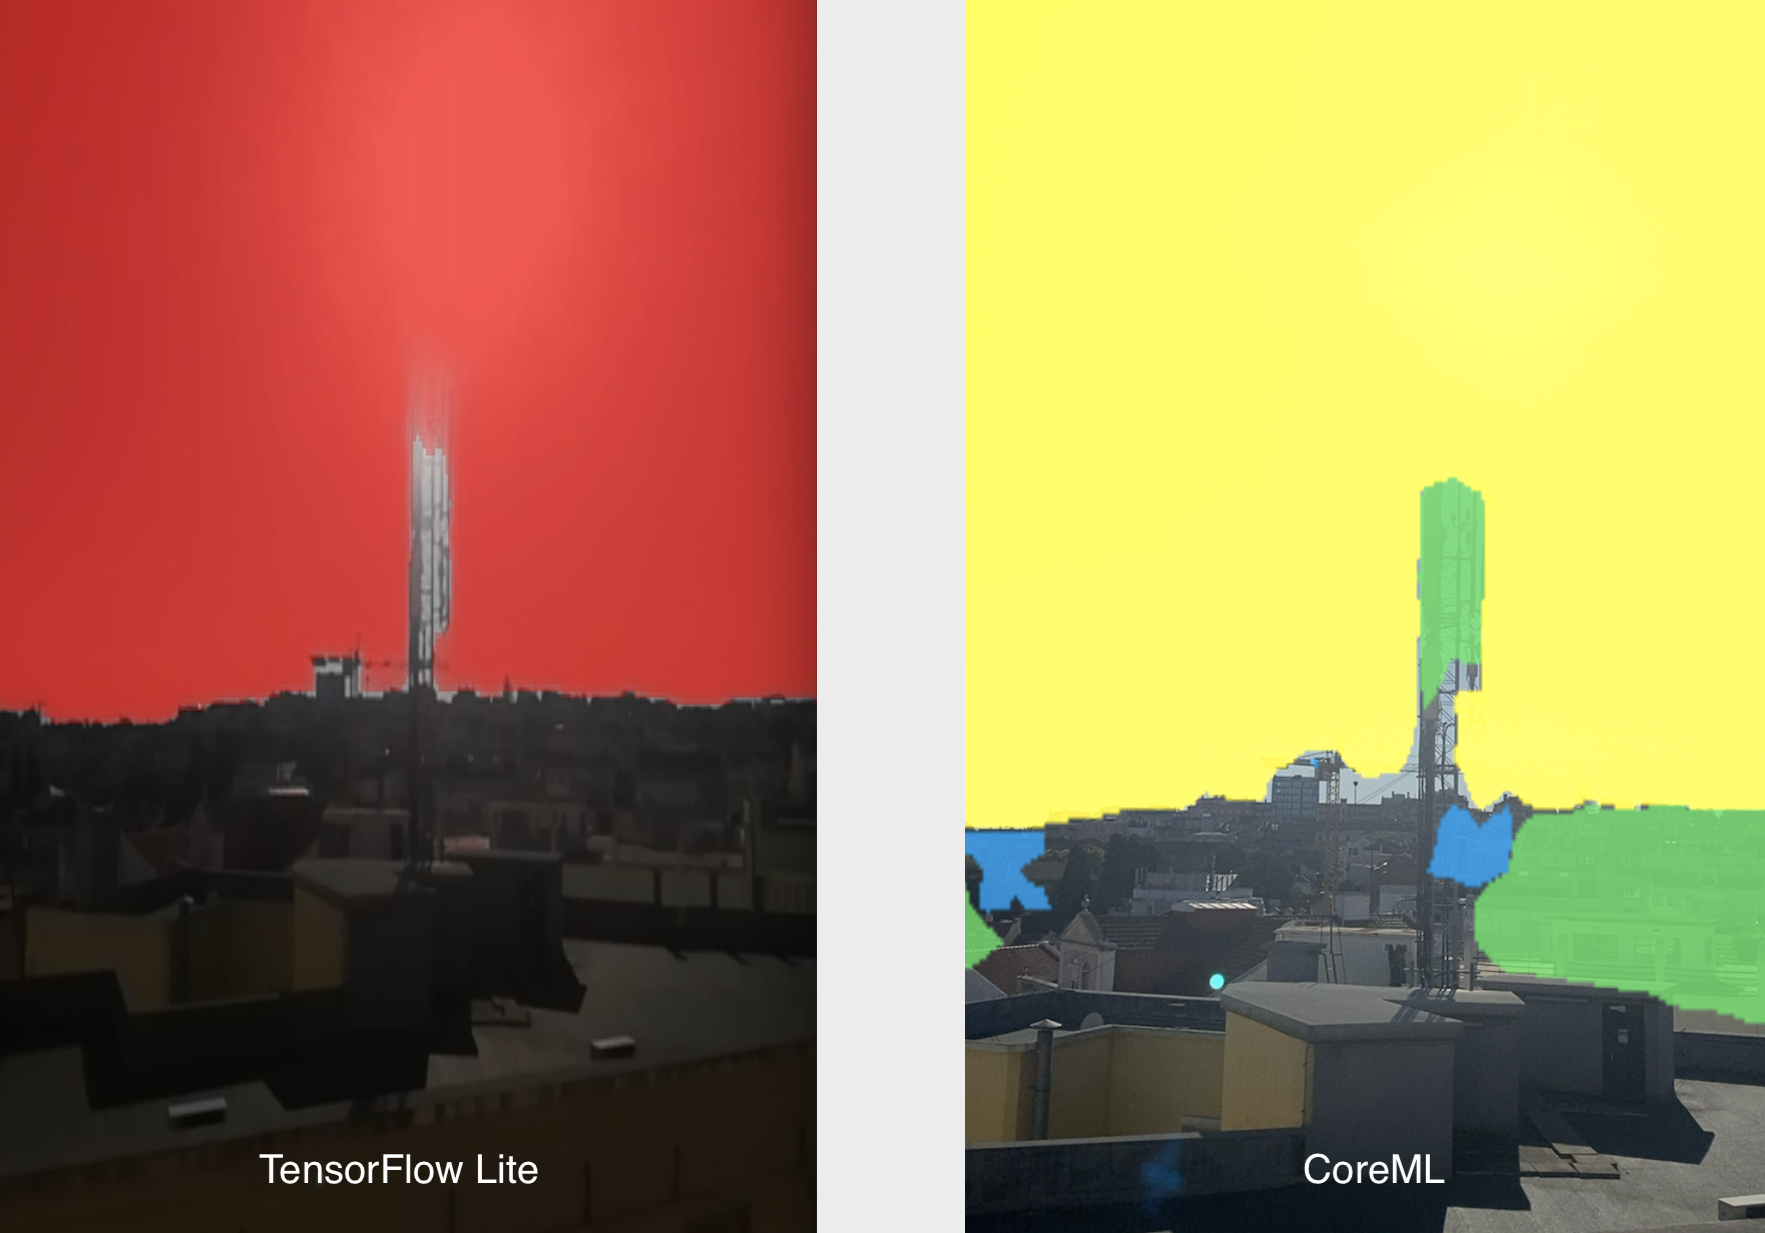
\includegraphics[scale=0.4]{SkySegmentation.png}
	\caption{Test luchtsegmentatie, zonder foutaanduiding}
\end{figure}

De test om de uitkomst van luchtsegmentatie te bekomen werd uitgevoerd in Lissabon in een hotelkamer. Het uitzicht bevat een antenne die de algoritmen een extra moeilijkheid zou kunnen bezorgen bij het uitvoeren van dit experiment, de resultaten zijn dan ook zeer interessant. In de onderstaande foto kan men de foute zones waarnemen, deze worden  aangegeven door middel van de roze zones. Men kan ook alvast opmerken dat de beeldkwaliteit van de camera een grote rol speelt bij dit experiment, de Core. De zeer kleine vlakken tussen de spaken van de antennen zorgen voor foute resultaten. Hieruit kan men bepalen dat het voor beide frameworks moeilijk is om zeer kleine vlakken te koppelen aan een bepaald segment. Dit visueel redeneringsproces werd ook 29 maal herhaald, en ook hier werd een puntensysteem gebruikt om de eindwinnaar te bepalen. In elke test kreeg het framework met het minste aantal foute zones een punt, het framework met het meeste punten na de 29ste test werd bekroond als 'winnaar' van dit deelexperiment. Uit de resultaten van dit deelexperiment kan men dus verder bepalen of de frameworks voldoen aan de nodige aspecten op vlak van nauwkeurig -en correctheid..
\begin{figure}[H]
	\centering
	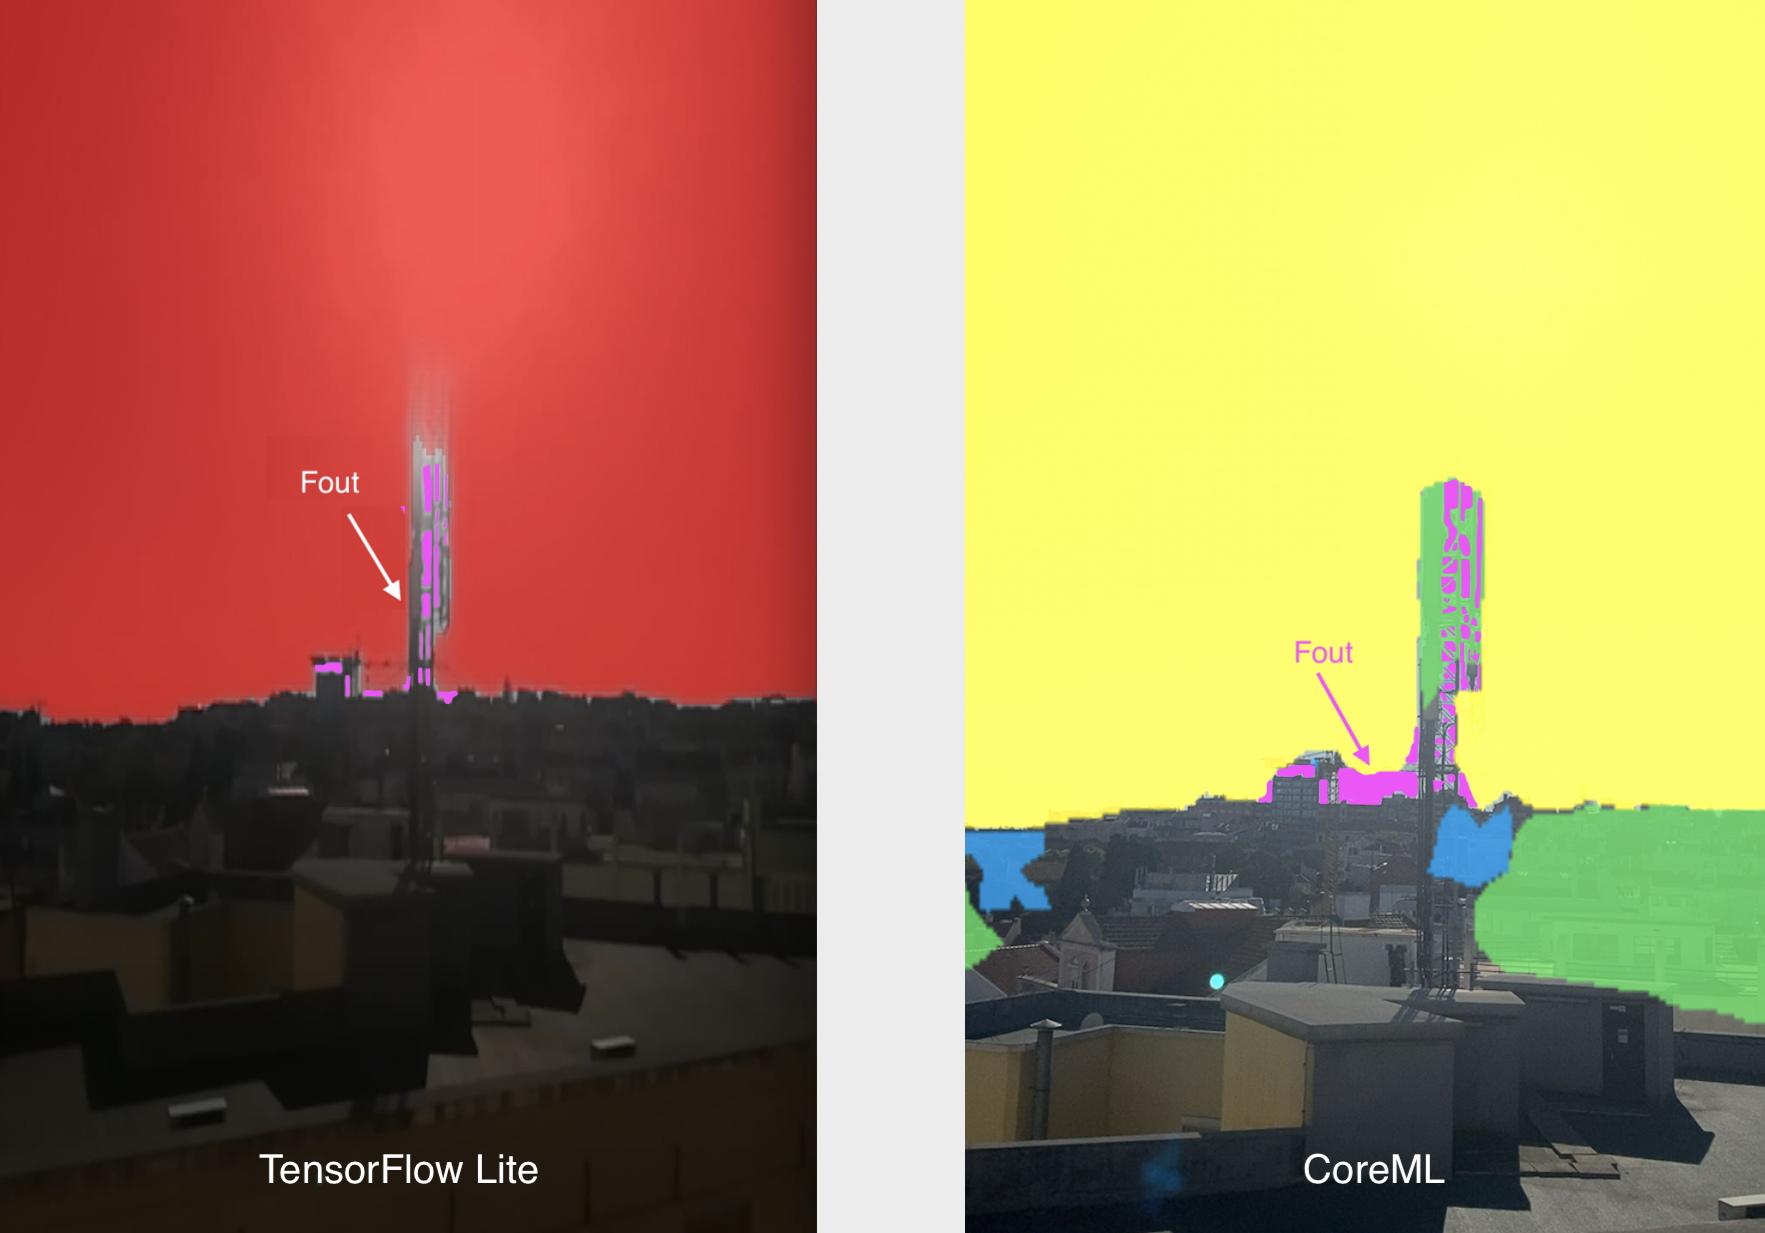
\includegraphics[scale=0.4]{SkySegmentation_MetFoutAanduiding.png}
	\caption{Test luchtsegmentatie, met foutaanduiding}
\end{figure}


\subsection{Segmentatie binnen gebouwen}
Segmentatie binnen gebouwen is de AI-eigenschap die het meeste zal doorwegen in het bepalen van het eindresultaat. De informatie die men uit dit experiment kan vergaren leunt het dichtste bij wat men nodig heeft om de wayfinding context te optimaliseren. Ten eerste is het zeer interessant om te zien hoe de AI-frameworks zullen reageren op de experimenten. Ten tweede is het ook zeer belangrijk om te weten of de bepaalde frameworks de muren of vloer binnen de opgegeven ruimte kan ontdekken + aanduiden. 

Tijdens het exploratief onderzoek was het niet vanzelfsprekend om twee uitgewerkte voorbeelden (TensorFlow Lite + CoreML) te vinden die gebruik maakten van dezelfde dataset. Daarom is het  experiment als volgt te werk gegaan, men testte twee uitgewerkte voorbeelden die elk een verschillende dataset utiliseerden. Men kan deze twee testresultaten dus niet rechtstreeks tegenover elkaar zetten. Alsnog kan men deze vergelijken met elkaar als men evalueert hoe goed beide frameworks in hun opzet zijn geslaagd. Het CoreML-framework werd getest door middel van de 'Fritz AI Studio' applicatie, deze maakt gebruik van een dataset die werd samengesteld door 'Fritz AI', de applicatie zal de volledige ruimte in kaart proberen brengen door middel van verschillende kleurvlekken. TensorFlow Lite werd getest door de 'Tiramisu' applicatie die werd gecreërd door Christian Kauten, deze applicatie is vooral gericht op het herkennen van de grond. Beide tests werden uitgevoerd met een iPhone 11. (camera: 12MP). 

Om deze AI-eigenschap zo optimaal mogelijk te evalueren heeft men beide frameworks getest op 3 verschillende plaatsen, deze plaatsen werden eerder aangegeven in Figuur 3.2 in de methodologie.

\subsubsection{Test 1}
\begin{figure}[H]
	\centering
	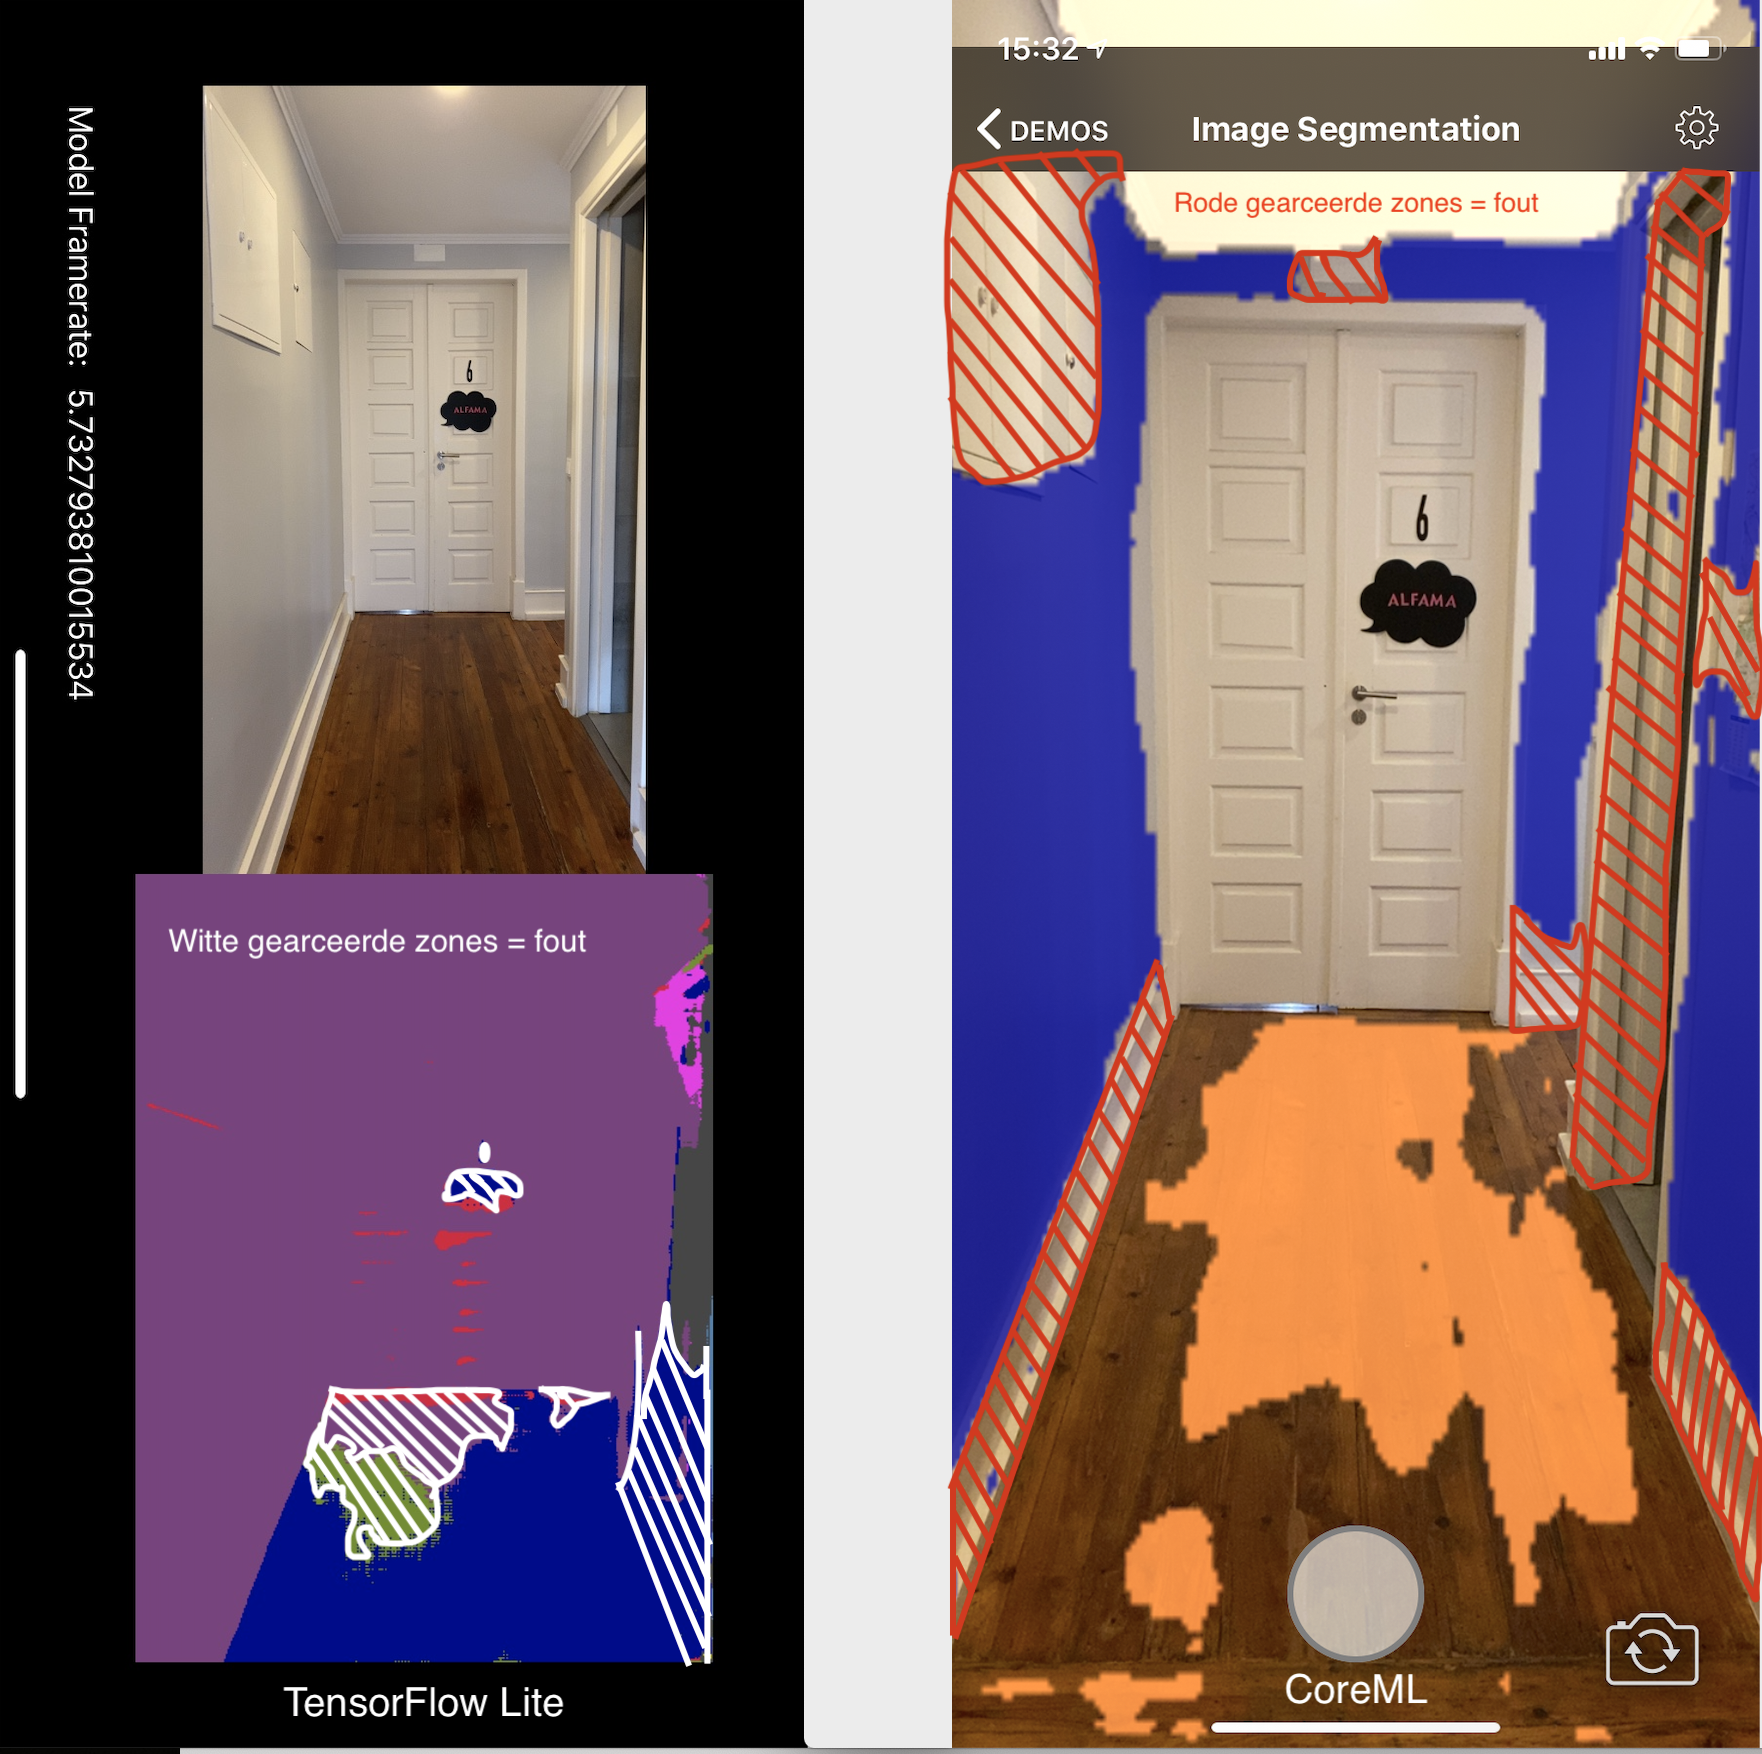
\includegraphics[scale=0.325]{ImageSegmentation_1.png}
	\caption{Test 1: TensorFlow Lite (links) \& CoreML (rechts)}
\end{figure}

De bovenstaande afbeelding toont hoe de eerste test is verlopen. Het TensorFlow Lite-framework zal in deze test zich focussen op het herkennen van grondoppervlaktes, het model is zo getrained. Het CoreML-framework is beter getrained, zoals men kan zien in de bovenstaande afbeelding kan dit framework de grond en muren detecteren, men zal zich voor dit framework vooral focussen op het detecteren van muren, de muurdetectie wordt als extra voordeel beschouwd.

De gearceerde zones (wit voor TensorFlow Lite, rood voor CoreML) tonen aan welke plaatsen men niet kon detecteren, maar wel moesten gedetecteerd worden. Zoals men eerder heeft vermeld worden deze twee tests niet rechstreeks met elkaar vergeleken, als men het aantal gearceerde zones kritiekloos met elkaar zou vergelijken, dan zou dit voor verkeerde resultaten zorgen. Men kan namelijk constateren dat er veel meer muuroppervlaktes zijn dan grondoppervlaktes, de kans dat er dus meer fouten optreden bij het herkennen van de muren is dus groter.

Dit redeneringsproces werd 29 keer herhaald, op deze manier kan men de consistentie van de frameworks testen,  'beginnersgeluk' wordt op deze manier vermeden. In elke iteratie werd gekeken welk framework het beste kon presteren in zijn doelopdracht, voor TensorFlow Lite ging men dus kijken hoeveel grondoppervlakte men kon herkennen, hetzelfde werd bij CoreML gedaan, maar dan met betrekking to muurherkenning. Het framework die het beste kon presteren kreeg in elke iteratie een punt. Na de 29ste iteratie werd gekeken welk framework de meeste punten had.

\subsubsection{Test 2}
\begin{figure}[H]
	\centering
	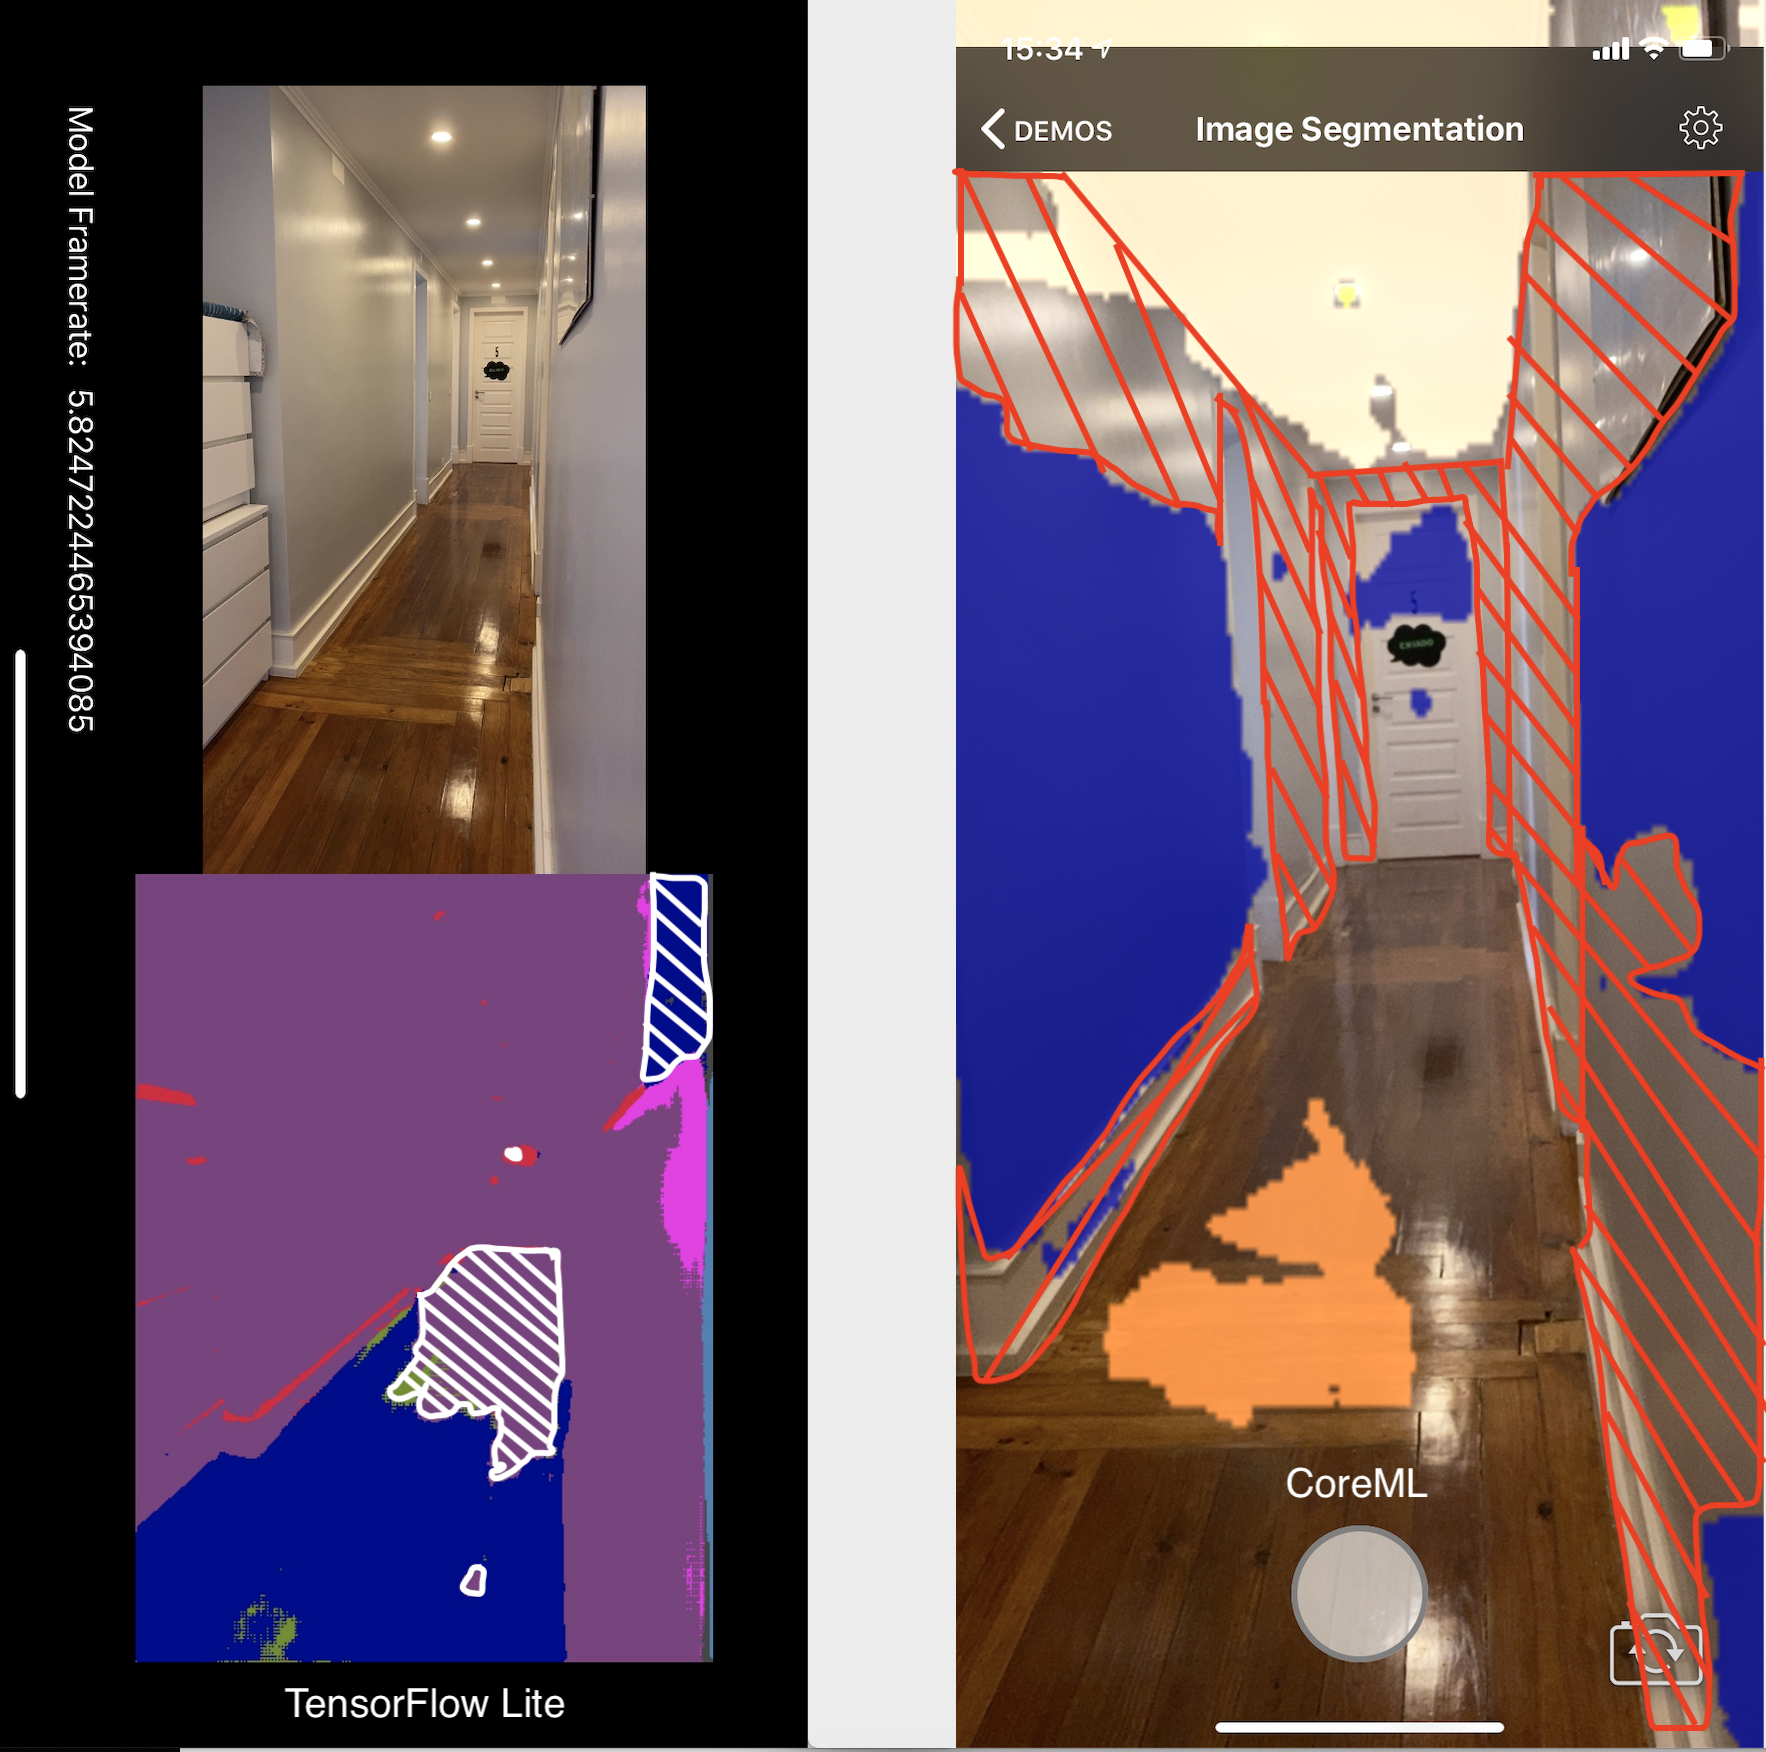
\includegraphics[scale=0.35]{ImageSegmentation_3.png}
	\caption{Test 2: TensorFlow Lite (links) \& CoreML (rechts)}
\end{figure}
De tweede test verliep op dezelfde manier als de eerste (zie bovenstaande foto), alleen de locatie werd gewijzigd. Deze test werd uitgevoerd in een langere gang, op deze manier kon men testen of de frameworks ook het grondoppervlak en de muren kon herkennen die zich verder begeefden. 

Ook in deze test werd er gekeken naar de foute gearceerde zones (wit voor TensorFlow Lite, rood voor CoreML). De regels die werden toegepast in de eerste test werden ook gebruikt in deze test, men kan in dit voorbeeld namelijk ook opmerken dat er veel meer muren aanwezig zijn als grond.

In deze test kan men duidelijk constateren dat het TensorFlow Lite-framework een beter resultaat oplevert als CoreML. CoreML slaagt in de voorbeeld er niet in om het grootste deel van de muren aan te duiden. Dit redeneringsproces werd zoals de andere testen reeds 29 keer herhaald, de evaluatie verliep op dezelfde wijze als de eerste test.

\subsubsection{Test 3}
\begin{figure}[H]
	\centering
	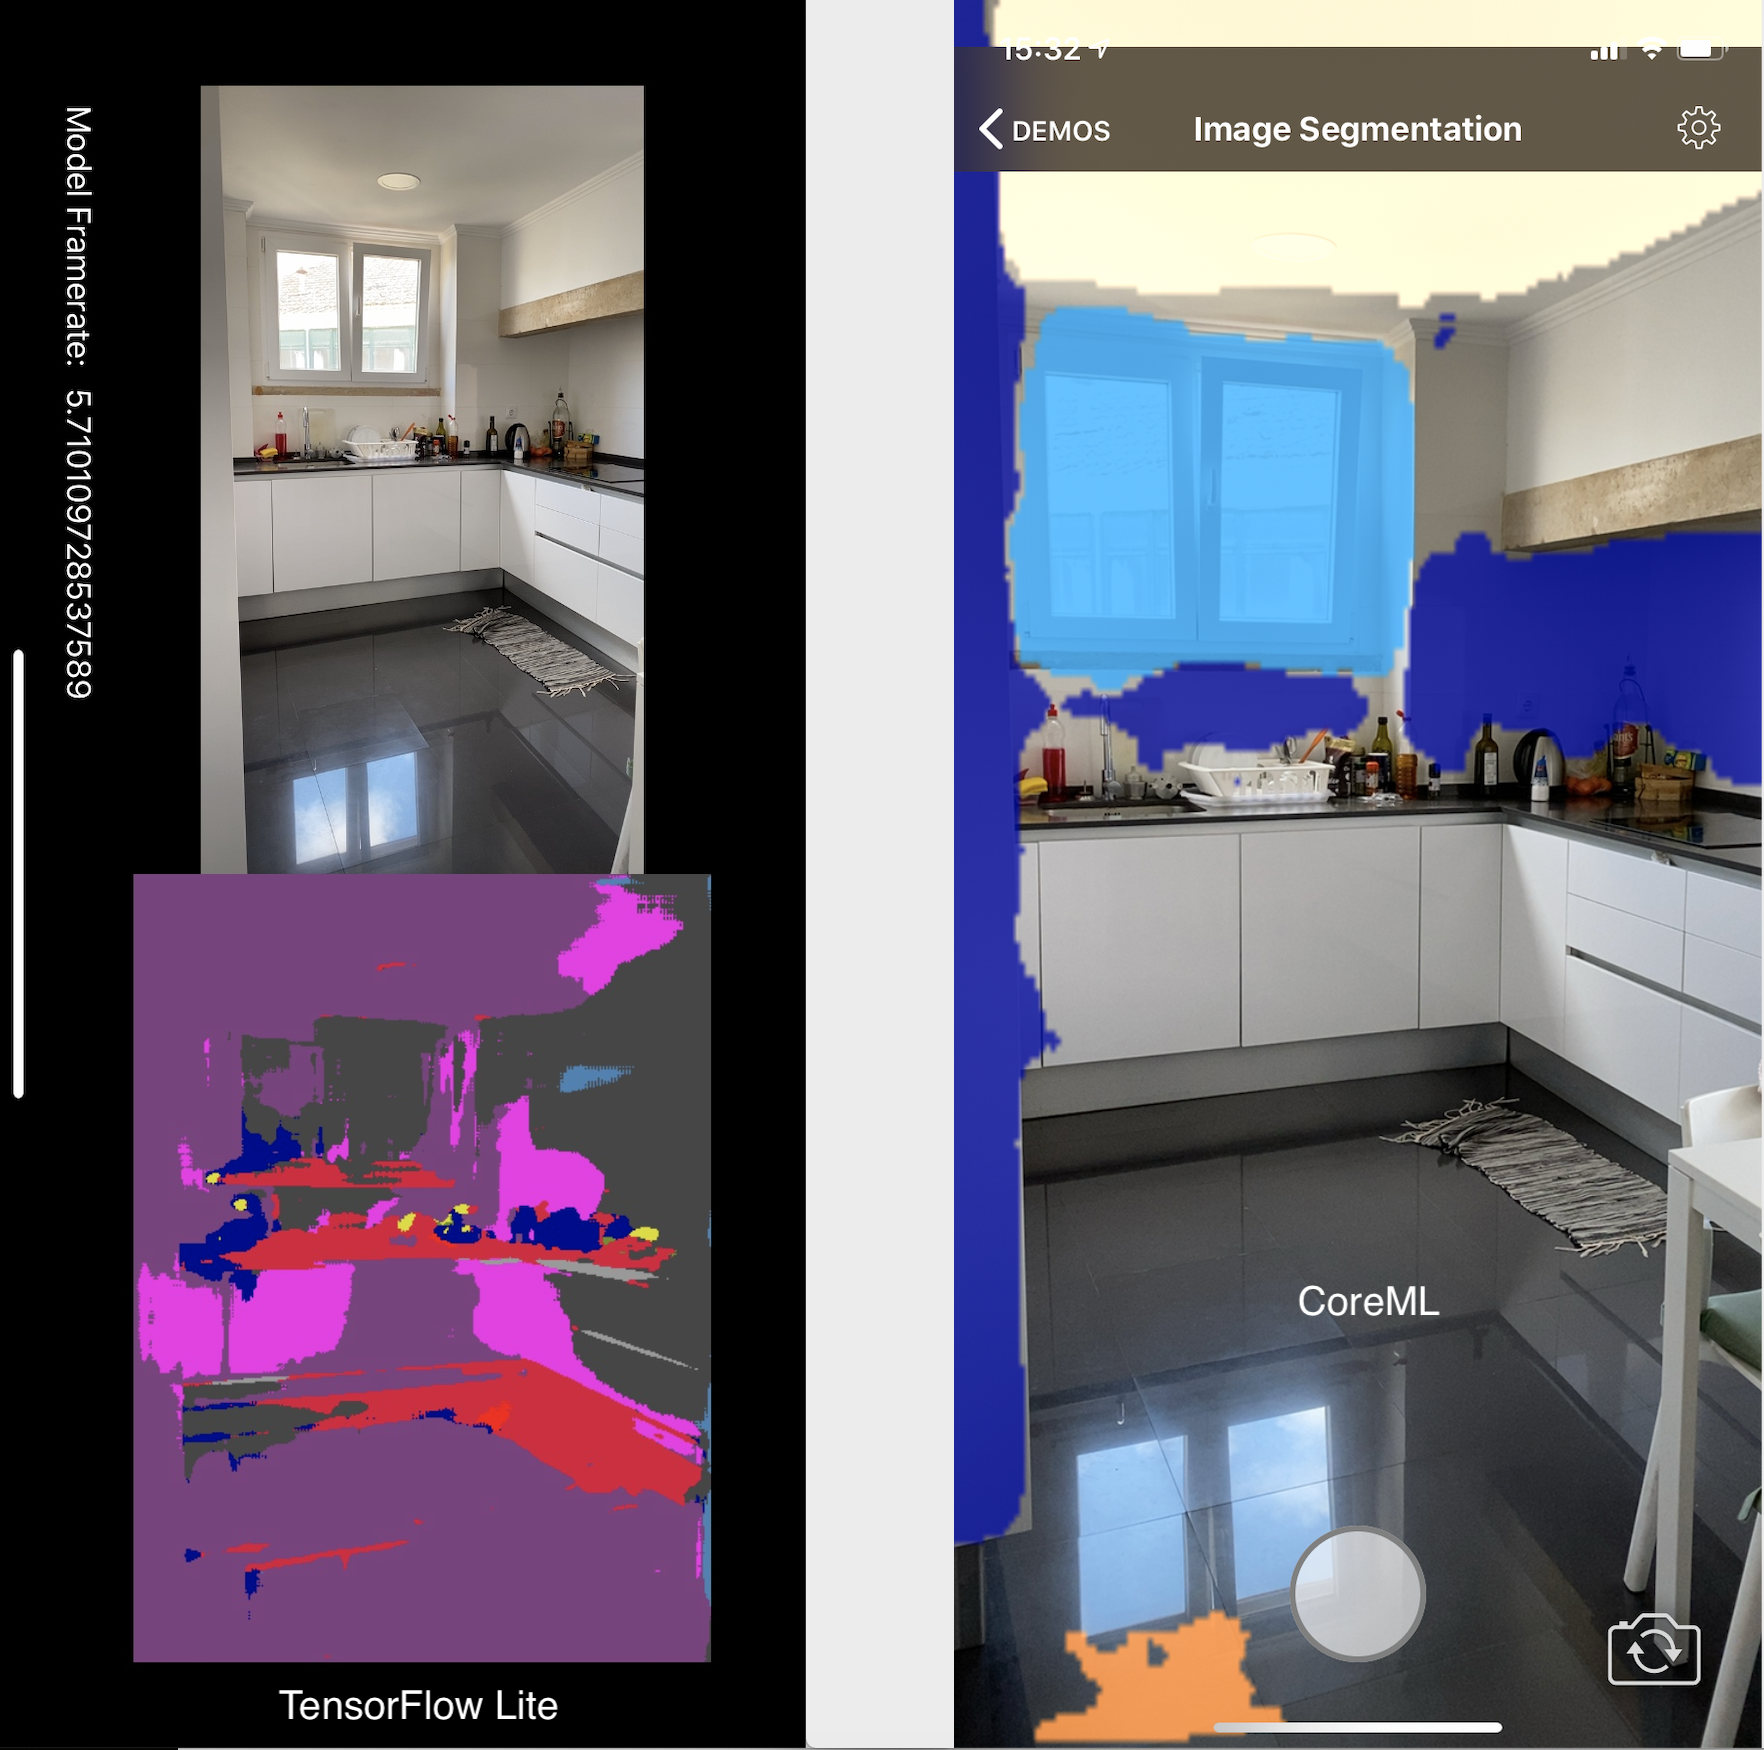
\includegraphics[scale=0.35]{ImageSegmentation_2.png}
	\caption{Test 2: TensorFlow Lite (links) \& CoreML (rechts)}
\end{figure}

Om deze AI-eigenschap op een zo optimaal mogelijk manier te testen werd het derde experiment op een locatie uitgevoerd die niets gemeenschappelijk had met de vorige tests. De derde test werd uitgevoerd in een keuken, deze locatie bevat veel verschillende objecten die voor storing zouden kunnen zorgen. De resultaten in het bovenstaande voorbeeld zijn dan ook opmerkelijk.

Om de resultaten te evalueren werd ook in dit voorbeeld gebruik gemaakt van foute zones die werden aangegeven door gearceerde vlekken. (wit voor TensorFlow Lite, rood voor CoreML). Men kan in dit voorbeeld constateren dat het TensorFlow Lite-framework er helemaal niet in slaagt om de grond te detecteren, een mogelijke factor is het weerkaatsen van het licht in de donkere stenen. Het resultaat van het CoreML-framework kent een beter resultaat, dit framework slaagt er wel degelijk in om de muren grotendeels te detecteren en aan te duiden. Ook deze test werd 29 maal herhaald, de regels uit de vorige twee testen werden hier ook toegepast. In dit voorbeeld zou het CoreML-framework een punt verdienen.

\chapter{\IfLanguageName{dutch}{Resultaten}{Results}}
\label{ch:resultaten}

In dit hoofdstuk zal men de resultaten bespreken van de uitgevoerde testen, dit zal worden gedaan met behulp van grafieken om het overzicht te bewaren. De resultaten zullen eerst worden besproken per AI-eigenschap, op het einde van dit hoofdstuk zal men een algemene conclusie vormen.

\section{Objectdetectie}

\subsection{Test met boek}
De resultaten van de eerste objectdetecttest zijn opmerkelijk, er is namelijk een zeer groot verschil tussen de 2 frameworks. CoreML haalde een gemiddelde van 88.9 \% (standaardafwijking: 10.41) terwijl TensorFlow Lite maar een gemiddelde haalde van 53.83 \% (standaardafwijking: 3.41), dit wilt zeggen dat het TensorFlow Lite-framework slechts in 53 van de 100 gevallen het boek correct zal herkennen en detecteren. Men kan wel constateren dat het CoreML-framework minder consistent is, de verschillende metingen zijn namelijk heel verpreid.

\begin{figure}[H]
	\centering
	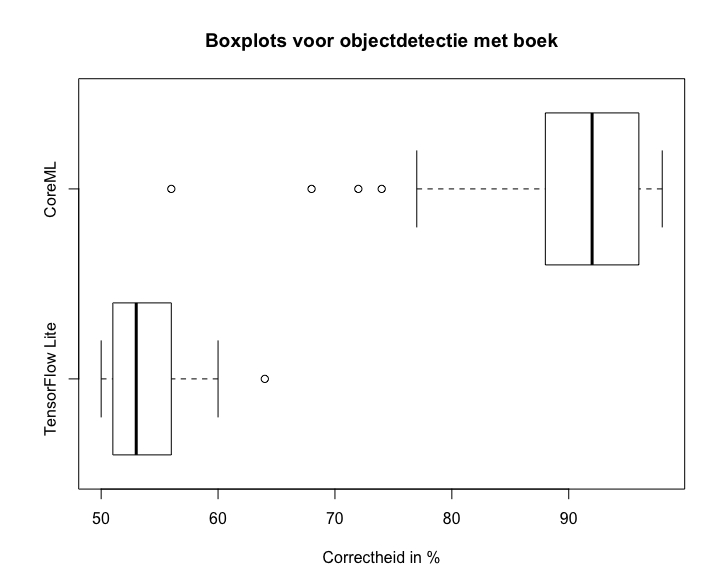
\includegraphics[scale=0.38]{Boxplots_Boek.png}
	\caption{Boxplots test boek}
\end{figure}
\subsection{Test met persoon}

De tweede test bracht eveneens zeer opmerkelijke resultaten, in de onderstaande boxplot kan men opmerken dat het CoreML-framework in bijna alle gevallen de persoon in kwestie met 100 \% zekerheid kon aanduiden. Het framework dat door TensorFlow wordt aangeboden scoort hier ook goed met een gemiddelde van 80 \% (standaardafwijking: 2.51). CoreML haalde in deze test een gemiddelde van 99.78 \% (standaardafwijking: 0.42), de lage waarde voor de standaardafwijking vertaalt zich in een zeer goede consistentie.
\begin{figure}[H]
	\centering
	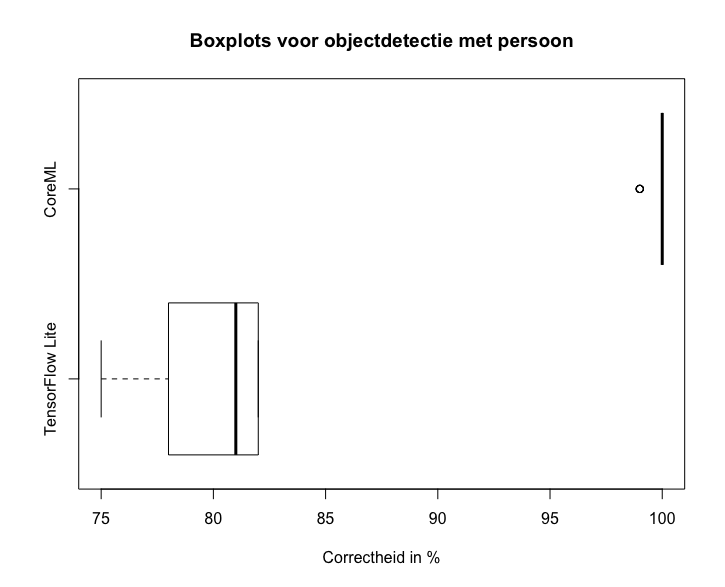
\includegraphics[scale=0.4]{Boxplots_Persoon.png}
	\caption{Boxplots test persoon}
\end{figure}

\subsection{Test met fles}
De derde zorgde voor gelijkaardige resultaten als de vorige tests. Opnieuw presteerde het CoreML-framework veel beter als TensorFlow Lite. Het framework van apple haalde een gemiddelde van 91.55 \% (standaardafwijking: 4.52), voor TensorFlow Lite bedraagde dit 58.89 \% (standaardafwijking: 3.65). Men kan andermaal concluderen dat beide frameworks consistente resultaten behaalden, dit is ook visueel zienbaar in de onderstaande boxplots. 
\begin{figure}[H]
	\centering
	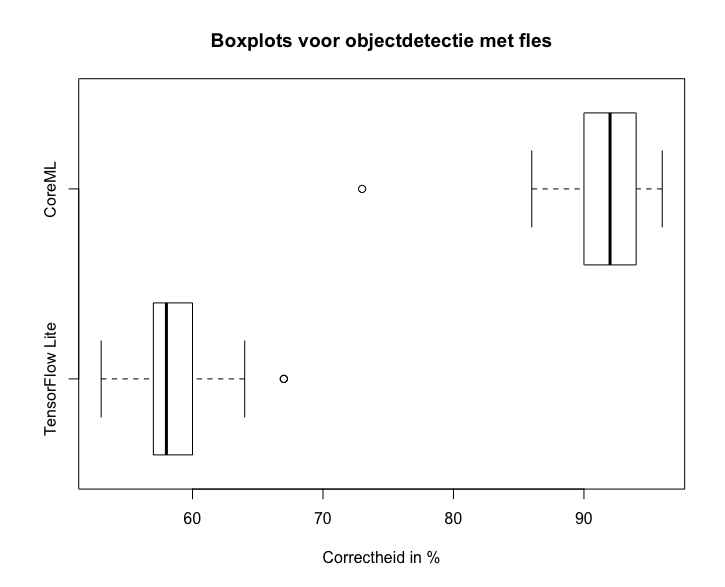
\includegraphics[scale=0.45]{Boxplots_Fles.png}
	\caption{Boxplots test fles}
\end{figure}
\subsection{Test met horloge}
De resultaten uit het vierde experiment zijn zeer interessant, opnieuw scoort het CoreML-framework betere resultaten dan TensorFlow Lite. CoreML haalde een gemiddelde van 78.55 \% (standaardafwijking: 13.38), TensorFlow lite behaalde 66.38 \% (standaardafwijking: 4.39). Op het eerste zicht lijkt CoreML de 'winnaar' in dit experiment, alsnog moet men dit in betwijfeling trekken. De consistentie van CoreML in dit experiment is zeer slecht, de resultaten fluctueren namelijk tussen de  56 en 95 \%. De hoge standaardafwijking is vervolgens ook visueel aantoonbaar op de onderstaande boxplot.
\begin{figure}[H]
	\centering
	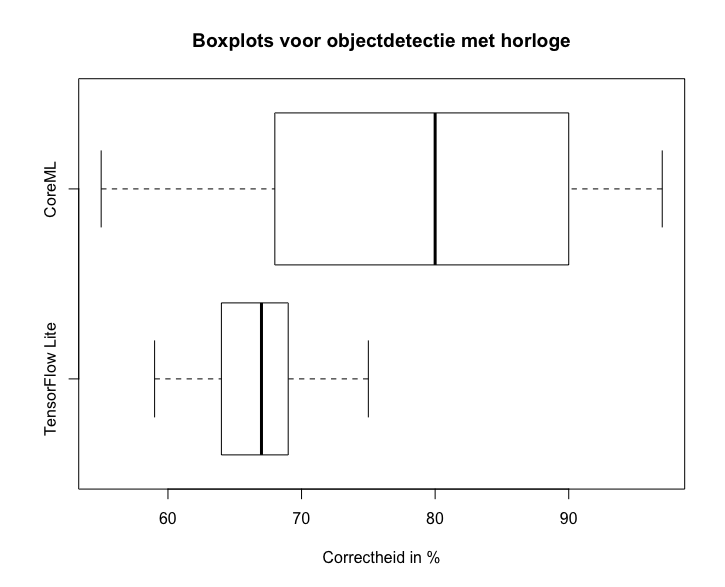
\includegraphics[scale=0.4]{Boxplots_Horloge.png}
	\caption{Boxplots test horloge}
\end{figure}
\subsection{Evaluatie}
In het algemeen kan men besluiten dat het CoreML-framework de beste  resultaten levert op vlak van objectdetectie. Men kan wel concluderen dat de hoge gemiddeldes vaak gepaard gaan met hoge standaardafwijkingen, dit betekent dat de consistentie lager is. In de onderstaande grafiek kan men telkens opnieuw zien dat CoreML ruim beter presteert. Zoals men eerder al heeft vermeld geeft deze AI-eigenschap een beter zicht over de nauwkeurig -en correctheid van het gebruikte algoritme.
\begin{figure}[H]
	\centering
	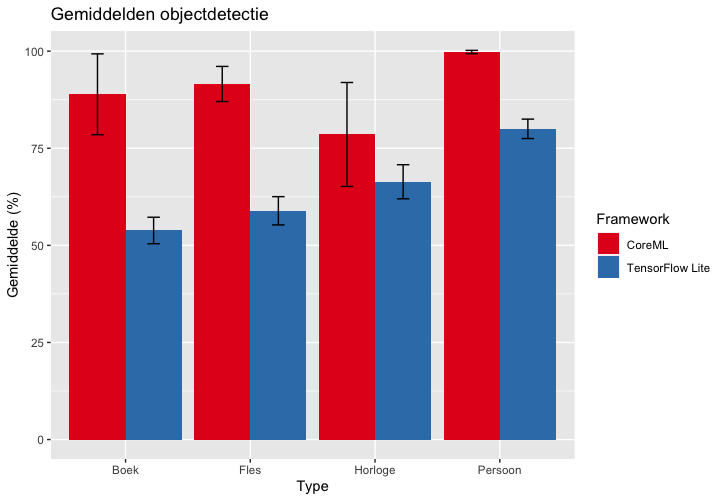
\includegraphics[scale=0.45]{Gemiddelde_objectdetectie.png}
	\caption{Gemiddelden objectdetectie}
\end{figure}

\section{Segmentatie}
\subsection{Menssegmentatie}
\begin{table}[H]
	\centering
	\begin{tabular}{|c|c|c|}
		\hline
		& \textbf{TensorFlow Lite} & \textbf{CoreML} \\ \hline
		\textbf{Aantal punten} & 3                        & 26              \\ \hline
	\end{tabular}
	\caption{Resultaten menssegmentatie test}
\end{table}

De resultaten uit de eerste segmentatietest zijn merkwaardig, CoreML haalt in deze test opnieuw de betere uitkomst. Het framework van Apple wist in 26 van de 29 een betere segmentatie uit zijn mouw te schudden. Het TensorFlow Lite-framework werkte niet nauwkeurig en gaf zeer vaak een compleet verkeerde output, CoreML slaagde er in om bijna elke test met minimale fouten af te werken.

\subsection{Luchtsegmentatie}
\begin{table}[H]
	\centering
	\begin{tabular}{|c|c|c|}
		\hline
		& \textbf{TensorFlow Lite} & \textbf{CoreML} \\ \hline
		\textbf{Aantal punten} & 7                        & 22              \\ \hline
	\end{tabular}
	\caption{Resultaten luchtsegmentatie test}
\end{table}

De tweede test werd op een simultane wijze uitgevoerd als de eerste, ook in deze test kan men zien dat CoreML betere prestaties levert. Men kan wel concluderen dat TensorFlow Lite een betere resultaat haalt als bij menssegmentatie. Alsnog kon men te veel fouten bespeuren in de resultaten van TensorFlow Lite. Bovendien was het CoreML-framework ook in staat om andere objecten binnen de afbeelding te segmenteren, ookal werden beide frameworks op dezelfde manier getrained.
\subsection{Segmentatie binnen gebouwen}

\subsubsection{Korte gang}
\begin{table}[H]
	\centering
	\begin{tabular}{|c|c|c|}
		\hline
		& \textbf{TensorFlow Lite} & \textbf{CoreML} \\ \hline
		\textbf{Aantal punten} & 3                        & 26              \\ \hline
	\end{tabular}
	\caption{Resultaten segmentatie binnen gebouwen: korte gang}
\end{table}
Zoals men eerder had beschreven werd de segmentatie binnen gebouwen op drie verschillende plaatsen getest. De resultaten van de eerste test zijn opnieuw zeer interessant. Opnieuw kan men significant verschil opmerken, het CoreML-framework slaagt er terug in om de beste resultaten te behalen. Ook tijdens het uitvoeren van de test kon men opmerken dat TensorFlow Lite een grondoppervlakt detecteerde die er in de werkelijkheid niet was, deze fouten zorgde voornamelijk voor het grote puntenverschil.

\subsubsection{Lange gang}
\begin{table}[H]
	\centering
	\begin{tabular}{|c|c|c|}
		\hline
		& \textbf{TensorFlow Lite} & \textbf{CoreML} \\ \hline
		\textbf{Aantal punten} & 9                        & 20              \\ \hline
	\end{tabular}
	\caption{Resultaten segmentatie binnen gebouwen: lange gang}
\end{table}
De resultaten van de test in de lange gang zijn ook zeer boeiend, deze test zou beproeven of de frameworks ook het grond -en muuroppervlak zouden detecteren over een langere afstand. Uit de resultaten kan men besluiten dat TensorFlow Lite opnieuw slechter presteert, maar in vergelijking met de vorige test kent men wel een groei. Opnieuw slaagt CoreML beter in zijn opzet, men kon wel een daling zien op vlak van prestaties tegenover de vorige test (in de korte gang).
\subsubsection{Keuken}

\begin{table}[H]
	\centering
	\begin{tabular}{|c|c|c|}
		\hline
		& \textbf{TensorFlow Lite} & \textbf{CoreML} \\ \hline
		\textbf{Aantal punten} & 0                        & 29              \\ \hline
	\end{tabular}
	\caption{Resultaten segmentatie binnen gebouwen: keuken}
\end{table}

\subsection{Evaluatie}
\begin{figure}[H]
	\centering
	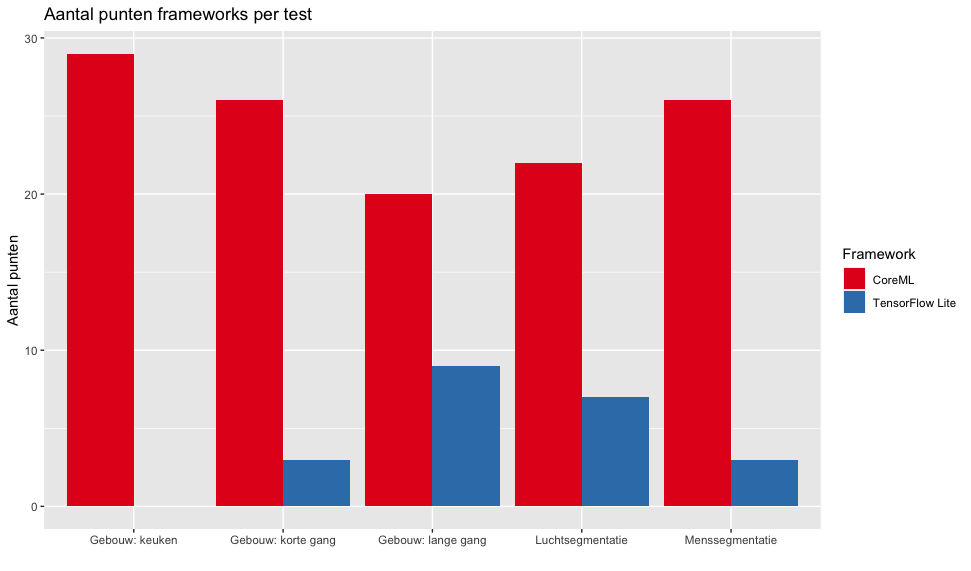
\includegraphics[scale=0.45]{Segmentatie_grafiek.png}
	\caption{Aantal punten per segmentatietest}
\end{figure}



